%%%%%%%%%%%%%%%%%%%%%%%%%%%%%%%%%%%%%%%%%%%%%%%%%
% Chapter: Tools
%%%%%%%%%%%%%%%%%%%%%%%%%%%%%%%%%%%%%%%%%%%%%%%%%
\chapter{Tools and Debuggers}
\label{chap:api_tools}

The term \textit{tool} widely refers to non-computational programs executed by the user or system administrator on a command line. Tools almost always interact with either the \ac{SMS}, user applications, or both to perform administrative and support functions. For example, a debugger tool might be used to remotely control the processes of a parallel application, monitoring their behavior on a step-by-step basis. Historically, such tools were custom-written for each specific host environment due to the customized and/or proprietary nature of the environment's interfaces.

The advent of \ac{PMIx} offers the possibility for creating portable tools capable of interacting with multiple \acp{RM} without modification. Possible use-cases include:

\begin{itemize}
\item querying the status of scheduling queues and estimated allocation time for various resource options
\item job submission and allocation requests
\item querying job status for executing applications
\item launching and monitoring applications
\end{itemize}

Enabling these capabilities requires some extensions to the \ac{PMIx} Standard (both in terms of \acp{API} and attributes), and utilization of client-side \acp{API} for more tool-oriented purposes.

This chapter defines specific \acp{API} related to tools, provides tool developers with an overview of the support provided by \ac{PMIx}, and serves to guide \ac{RM} vendors regarding roles and responsibilities of \acp{RM} to support tools. As the number of tool-specific \acp{API} and attributes is fairly small, the bulk of the chapter serves to provide a "theory of operation" for tools and debuggers. Description of the \acp{API} themselves is therefore deferred to the Section \ref{chap:api_tools:apis} later in the chapter.

%%%%%%%%%%%%%%%%%%%%%%%%%%%%%%%%%%%%%%%%%%%%%%
%%%%%%%%%%%%%%%%%%%%%%%%%%%%%%%%%%%%%%%%%%%%%%
\section{Connection Mechanisms}
\label{chap:api_tools:cnct}

The key to supporting tools lies in providing mechanisms by which a tool can connect to a \ac{PMIx} server. Application processes are able to connect because their local \ac{RM} daemon provides them with the necessary contact information upon execution. A command-line tool, however, isn't spawned by an \ac{RM} daemon, and therefore lacks the information required for rendezvous with a \ac{PMIx} server.

Once a tool has started, it initializes \ac{PMIx} as a tool (via \refapi{PMIx_tool_init}) if its access is restricted to \ac{PMIx}-based informational services such as \refapi{PMIx_Query_info}. However, if the tool intends to start jobs, then it must include the \refattr{PMIX_LAUNCHER} attribute to inform the library of that intent so that the library can initialize and provide access to the corresponding support.

Support for tools requires that the \ac{PMIx} server be initialized with an appropriate attribute indicating that tool connections are to be allowed. Separate attributes are provided to "fine-tune" this permission by allowing the environment to independently enable (or disable) connections from tools executing on nodes other than the one hosting the server itself. The \ac{PMIx} server library shall provide an opportunity for the host environment to authenticate and approve each connection request from a specific tool by calling the \refapi{pmix_server_tool_connection_fn_t} "hook" provided in the server module for that purpose. Servers in environments that do not provide this "hook" shall automatically reject all tool connection requests.

Tools can connect to any local or remote \ac{PMIx} server provided they are either explicitly given the required connection information, or are able to discover it via one of several defined rendezvous protocols. Connection discovery centers around the existence of \emph{rendezvous files} containing the necessary connection information, as illustrated in Fig. \ref{fig:rndvz}.

\begingroup
\begin{figure*}[ht!]
  \begin{center}
    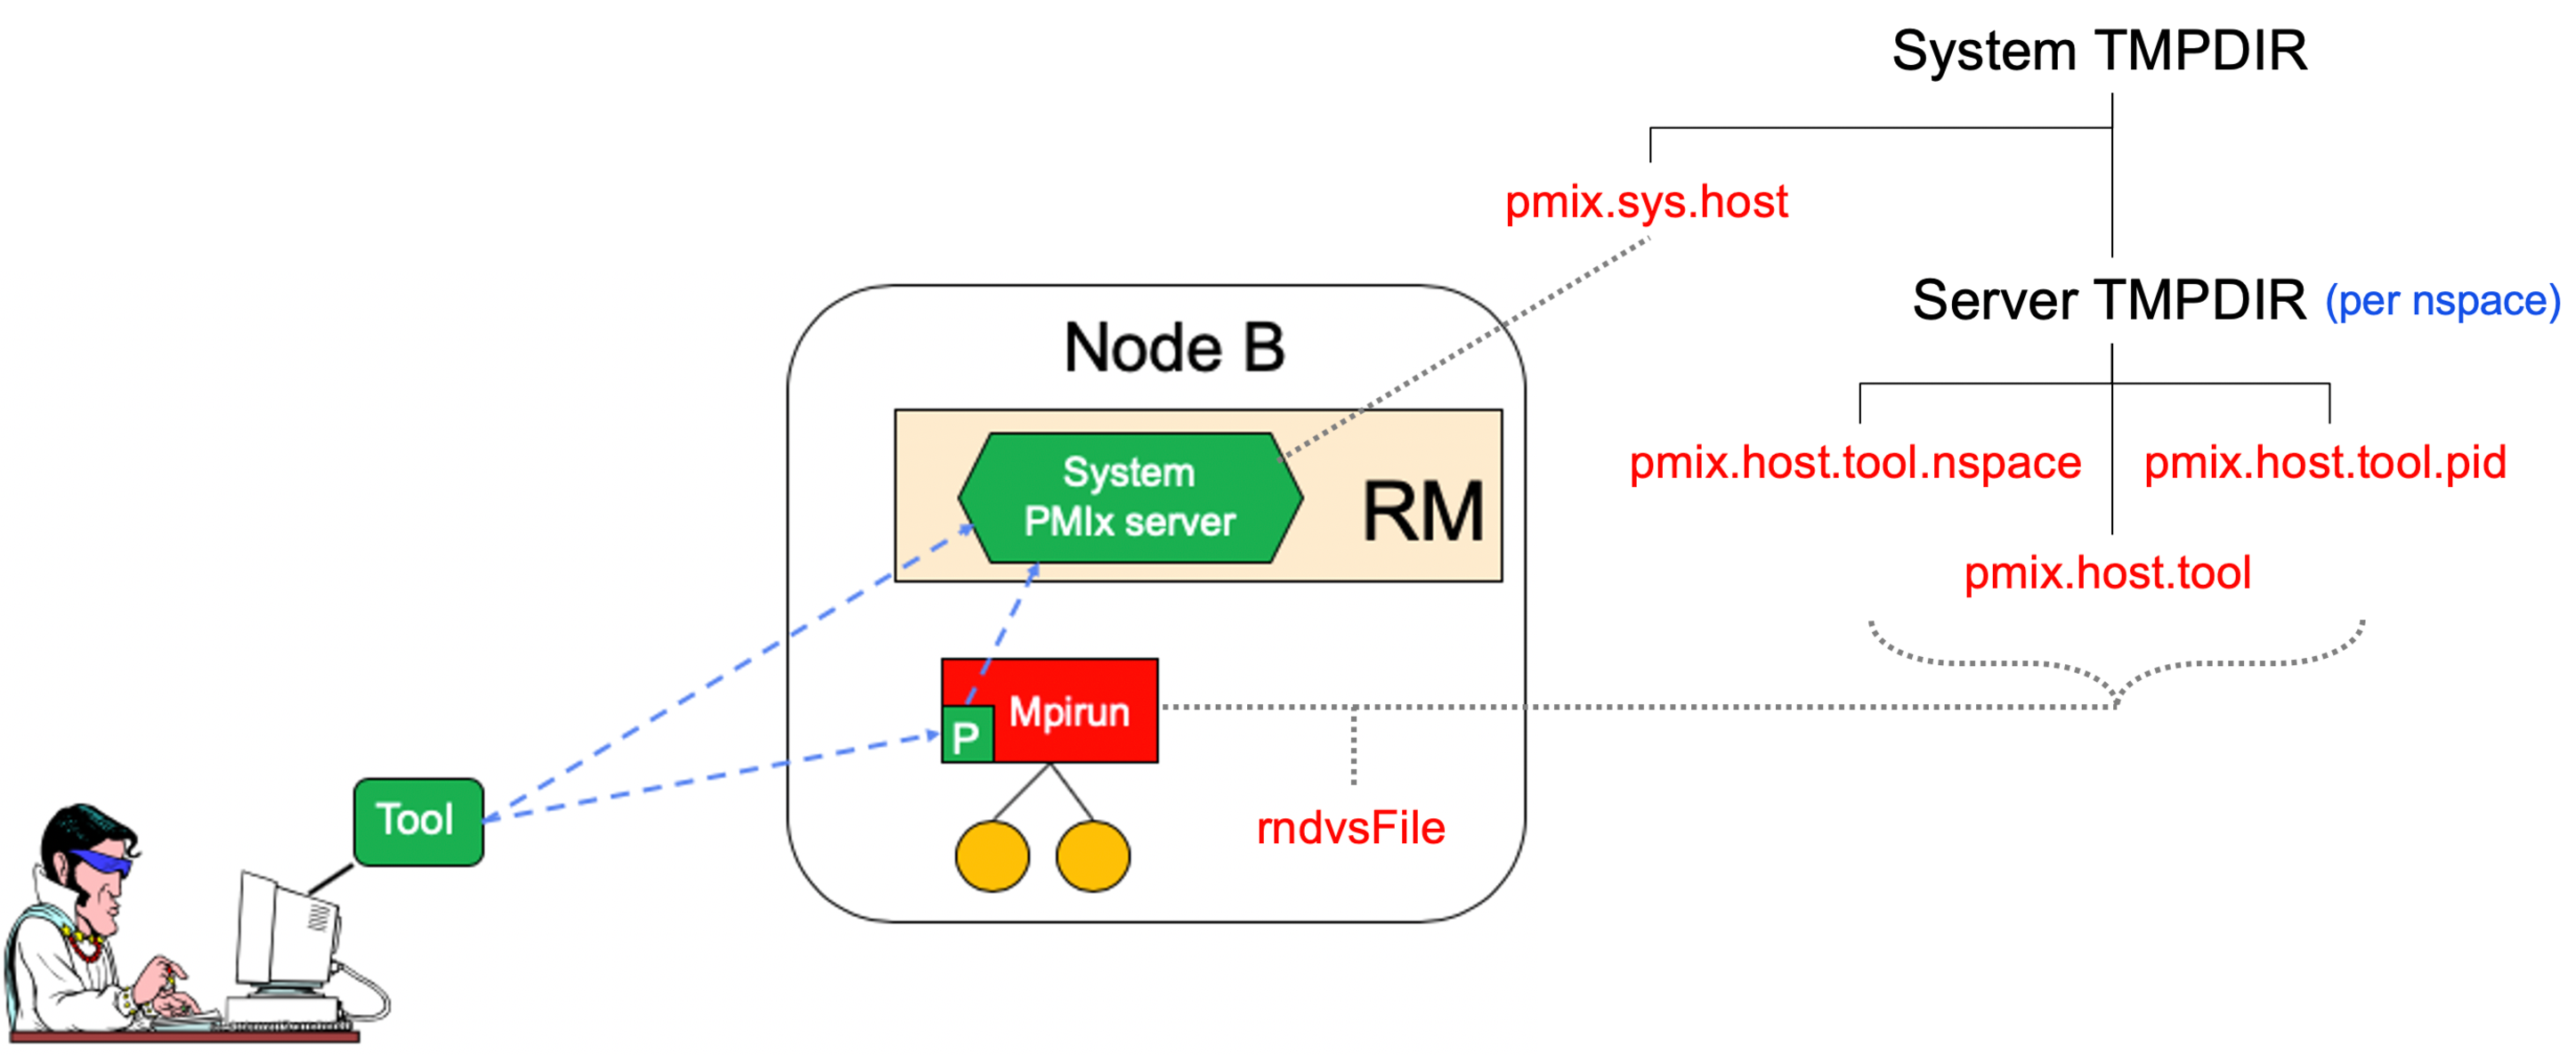
\includegraphics[clip,width=0.8\textwidth]{figs/rndvz.pdf}
  \end{center}
  \caption{Tool rendezvous files}
  \label{fig:rndvz}
\end{figure*}
\endgroup

The contents of each rendezvous file are specific to a given \ac{PMIx} implementation, but should at least contain the namespace and rank of the server along with its connection \ac{URI}. Note that tools linked to one \ac{PMIx} implementation are therefore unlikely to successfully connect to \ac{PMIx} server libraries from another implementation.

The top of the directory tree is defined by either the \refattr{PMIX_SYSTEM_TMPDIR} attribute (if given) or the \code{TMPDIR} environmental variable. \ac{PMIx} servers that are designated as \emph{system servers} by including the \refattr{PMIX_SERVER_SYSTEM_SUPPORT} attribute when calling \refapi{PMIx_server_init} will create a rendezvous file in this top-level directory. The filename will be of the form \emph{pmix.sys.hostname}, where \emph{hostname} is the string returned by the \code{gethostname} system call. Note that only one \ac{PMIx} server on a node can be designated as the system server.

Non-system \ac{PMIx} servers will create a set of three rendezvous files in the directory defined by either the \refattr{PMIX_SERVER_TMPDIR} attribute or the \code{TMPDIR} environmental variable:

\begin{itemize}
    \item \emph{pmix.host.tool.nspace} where \emph{host} is the string returned by the \code{gethostname} system call and \emph{nspace} is the namespace of the server
    \item \emph{pmix.host.tool.pid} where \emph{host} is the string returned by the \code{gethostname} system call and \emph{pid} is the \ac{PID} of the server
    \item \emph{pmix.host.tool}  where \emph{host} is the string returned by the \code{gethostname} system call. Note that servers which are not given a namespace-specific \refattr{PMIX_SERVER_TMPDIR} attribute may not generate this file due to conflicts should multiple servers be present on the node.
\end{itemize}

The files are identical and may be implemented as symlinks to a single instance. The individual file names are composed so as to aid the search process should a tool wish to connect to a server identified by its namespace or \ac{PID}.

Servers will additionally provide a rendezvous file in any given location if the path (either absolute or relative) and filename is specified either during \refapi{PMIx_server_init} using the \refattr{PMIX_LAUNCHER_RENDEZVOUS_FILE} attribute, or by the \code{PMIX_LAUNCHER_RENDEZVOUS_FILE} environmental variable prior to executing the process containing the server. This latter mechanism may be the preferred mechanism for tools such as debuggers that need to fork/exec a launcher (e.g., "mpiexec") and then rendezvous with it. This is described in more detail in Section \ref{chap:api_tools:indirect}.

Rendezvous file ownerships are set to the \ac{UID} and \ac{GID} of the server that created them, with permissions set according to the desires of the implementation and/or system administrator policy. All connection attempts are first governed by read access privileges to the target rendezvous file - thus, the combination of permissions, \ac{UID}, and \ac{GID} of the rendezvous files act as a first-level of security for tool access.

A tool may connect to as many servers at one time as the implementation supports, but is limited to designating only one such connection as its \emph{primary} server. This is done to avoid confusion when the tool calls an \ac{API} as to which server should service the request. The first server the tool connects to is automatically designated as the \emph{primary} server.

Tools are allowed to change their primary server at any time via the \refapi{PMIx_tool_set_server} \ac{API}, and to connect/disconnect from a server as many times as desired. Note that standing requests (e.g., event registrations) with the current primary server may be lost and/or may not be transferred when transitioning to another primary server - \ac{PMIx} implementors are not required to maintain or transfer state across tool-server connections.

Tool process identifiers are assigned by one of the following methods:

\begin{itemize}
    \item If \refattr{PMIX_TOOL_NSPACE} is given, then the namespace of the tool will be assigned that value
    \item If \refattr{PMIX_TOOL_RANK} is given, then the rank of the tool will be assigned that value. Passing \refattr{PMIX_TOOL_NSPACE} without also specifying the rank will result in the rank being set to a default value of zero
    \item If a process ID has not been provided, then one will be assigned by the host environment upon connection to a server. Users should note that the tool's process ID will be \emph{invalid} until a connection has been established
\end{itemize}

Tool process identifiers remain constant across servers. Thus, it is critical that a system-wide unique namespace be provided if the tool itself sets the identifier, and that host environments provide a system-wide unique identifier in the case where the identifier is set by the server upon connection. The host environment is required to reject any connection request that fails to meet this criterion.

For simplicity, the following descriptions will refer to the:

\begin{itemize}
    \item \code{PMIX_SYSTEM_TMPDIR} as the directory specified by either the \refattr{PMIX_SYSTEM_TMPDIR} attribute (if given) or the \code{TMPDIR} environmental variable.
    \item \code{PMIX_SERVER_TMPDIR} as the directory specified by either the \refattr{PMIX_SERVER_TMPDIR} attribute or the \code{TMPDIR} environmental variable
\end{itemize}

The rendezvous methods are automatically employed for the initial tool connection during \refapi{PMIx_tool_init} unless the \refattr{PMIX_TOOL_DO_NOT_CONNECT} attribute is specified, and on all subsequent calls to \refapi{PMIx_tool_connect_to_server}.

\subsection{Rendezvousing with a local server}

Connection to a local \ac{PMIx} server is pursued according to the following precedence chain based on attributes contained in the call to the \refapi{PMIx_tool_init} or \refapi{PMIx_tool_connect_to_server} \acp{API}. Servers to which the tool already holds a connection will be ignored. Except where noted, the \ac{PMIx} library will return an error if the specified file cannot be found, the caller lacks permissions to read it, or the server specified within the file does not respond to or accept the connection — the library will not proceed to check for other connection options as the user specified a particular one to use.

\begin{itemize}

\item If \refattr{PMIX_TOOL_ATTACHMENT_FILE} is given, then the tool will attempt to read the specified file and connect to the server based on the information contained within it.

\item If \refattr{PMIX_SERVER_URI} or \refattr{PMIX_TCP_URI} is given, then connection will be attempted to the server at the specified \ac{URI}. Note that it is an error for both of these attributes to be specified. \refattr{PMIX_SERVER_URI} is the preferred method as it is more generalized — \refattr{PMIX_TCP_URI} is provided for those cases where the user specifically wants to use a \ac{TCP} transport for the connection and wants to error out if one isn’t available or cannot be used.

\item If \refattr{PMIX_SERVER_PIDINFO} was provided, then the tool will search for a rendezvous file created by a \ac{PMIx} server of the given \ac{PID} in the \code{PMIX_SERVER_TMPDIR} directory..

\item If \refattr{PMIX_SERVER_NSPACE} is given, then the tool will search for a rendezvous file created by a \ac{PMIx} server of the given namespace in the \code{PMIX_SERVER_TMPDIR} directory.

\item If \refattr{PMIX_CONNECT_TO_SYSTEM} is given, then the tool will search for a system-level rendezvous file created by a \ac{PMIx} server in the \code{PMIX_SYSTEM_TMPDIR} directory.

\item If \refattr{PMIX_CONNECT_SYSTEM_FIRST} is given, then the tool will look for a system-level rendezvous file created by a \ac{PMIx} server in the \code{PMIX_SYSTEM_TMPDIR} directory. If found, then the tool will attempt to connect to it. In this case, no error will be returned if the rendezvous file is not found or connection is refused — the \ac{PMIx} library will silently continue to the next option

\item By default, the tool will search the directory tree under the \code{PMIX_SERVER_TMPDIR} directory for rendezvous files of \ac{PMIx} servers, attempting to connect to each it finds until one accepts the connection. If no rendezvous files are found, or all contacted servers refuse connection, then the \ac{PMIx} library will return an error.
\end{itemize}

Note that there can be multiple local servers - one from the system plus others from launchers and active jobs. The \ac{PMIx} tool connection search method is not guaranteed to pick a particular server unless directed to do so.


\subsection{Connecting to a remote server}

Connecting to remote servers is complicated due to the lack of access to the previously-described rendezvous files. Two methods are required to be supported, both based on the caller having explicit knowledge of either connection information or a path to a local file that contains such information:


\begin{itemize}

\item If \refattr{PMIX_TOOL_ATTACHMENT_FILE} is given, then the tool will attempt to read the specified file and connect to the server based on the information contained within it.

\item If \refattr{PMIX_SERVER_URI} or \refattr{PMIX_TCP_URI} is given, then connection will be attempted to the server at the specified \ac{URI}. Note that it is an error for both of these attributes to be specified. \refattr{PMIX_SERVER_URI} is the preferred method as it is more generalized — \refattr{PMIX_TCP_URI} is provided for those cases where the user specifically wants to use the \ac{TCP} transport for the connection and wants to error out if it isn’t available or cannot be used.

\end{itemize}

Additional methods may be provided by particular \ac{PMIx} implementations. For example, the tool may use \emph{ssh} to launch a \emph{probe} process onto the remote node so that the probe can search the \code{PMIX_SYSTEM_TMPDIR} and \code{PMIX_SERVER_TMPDIR} directories for rendezvous files, relaying the discovered information back to the requesting tool. If sufficient information is found to allow for remote connection, then the tool can use it to establish the connection. Note that this method is not required to be supported - it is provided here as an example and left to the discretion of \ac{PMIx} implementors.


\subsection{Attaching to running jobs}

When attaching to a running job, the tool must connect to a \ac{PMIx} server that is associated with that job - e.g., a server residing in the host environment's local daemon that spawned one or more of the job's processes, or the server residing in the launcher that is overseeing the job. Identifying an appropriate server can sometimes prove challenging, particularly in an environment where multiple job launchers may be in operation, possibly under control of the same user.

In cases where the user has only the one job of interest in operation on the local node (e.g., when engaged in an interactive session on the node from which the launcher was executed), the normal rendezvous file discovery method can often be used to successfully connect to the target job, even in the presence of jobs executed by other users. The permissions and security authorizations can, in many cases, reliably ensure that only the one connection can be made. However, this is not guaranteed in all cases.

The most common method, therefore, for attaching to a running job is to specify either the \ac{PID} of the job's launcher or the namespace of the launcher's job (note that the launcher's namespace frequently differs from the namespace of the job it has launched). Unless the application processes themselves act as \ac{PMIx} servers, connection must be to the servers in the daemons that oversee the application. This is typically either daemons specifically started by the job's launcher process, or daemons belonging to the host environment, that are responsible for starting the application's processes and oversee their execution.

Identifying the correct \ac{PID} or namespace can be accomplished in a variety of ways, including:

\begin{itemize}
    \item Using typical \ac{OS} or host environment tools to obtain a listing of active jobs and perusing those to find the target launcher
    \item Using a \ac{PMIx}-based tool attached to a system-level server to query the active jobs and their command lines, thereby identifying the application of interest and its associated launcher
    \item Manually recording the \ac{PID} of the launcher upon starting the job
\end{itemize}

Once the namespace and/or \ac{PID} of the target server has been identified, either of the previous methods can be used to connect to it.


%%%%%%%%%%%
\subsection{Tool initialization attributes}
\label{api:tools:attributes:tool}

The following attributes are passed to the \refapi{PMIx_tool_init} \ac{API} for use when initializing the \ac{PMIx} library.

%
\declareAttribute{PMIX_TOOL_NSPACE}{"pmix.tool.nspace"}{char*}{
Name of the namespace to use for this tool.
}

%
\declareAttribute{PMIX_TOOL_RANK}{"pmix.tool.rank"}{uint32_t}{
Rank of this tool.
}

%
\declareAttribute{PMIX_LAUNCHER}{"pmix.tool.launcher"}{bool}{
Tool is a launcher and needs to create rendezvous files
}

%%%%%%%%%%%
\subsection{Tool initialization environmental variables}
\label{api:tools:envars:tool}

The following environmental variables are used during \refapi{PMIx_tool_init} to control various rendezvous-related operations when the tool is started manually (e.g., on a command line) or by a fork/exec-like operation.

%
\declareNewEnvar{PMIX_LAUNCHER_PAUSE_FOR_TOOL}{
Upon completing \refapi{PMIx_server_init}, the spawned launcher is to generate the \refconst{PMIX_LAUNCHER_READY} event and then pause until the spawning tool can connect to it and provide directives.
}

%
\declareNewEnvar{PMIX_LAUNCHER_RENDEZVOUS_FILE}{
Pathname of file where the launcher is to store its connection information so that the spawning tool can connect to it.
}

%%%%%%%%%%%
\subsection{Tool connection attributes}
\label{api:struct:attributes:connection}

These attributes are defined to assist PMIx-enabled tools to connect with a \ac{PMIx} server by passing them into either the \refapi{PMIx_tool_init} or the \refapi{PMIx_tool_connect_to_server} \acp{API} - thus, they are not typically accessed via the \refapi{PMIx_Get} \ac{API}.


%
\declareAttribute{PMIX_SERVER_PIDINFO}{"pmix.srvr.pidinfo"}{pid_t}{
\ac{PID} of the target PMIx server for a tool.
}

%
\declareAttribute{PMIX_CONNECT_TO_SYSTEM}{"pmix.cnct.sys"}{bool}{
The requester requires that a connection be made only to a local, system-level PMIx server.
}

%
\declareAttribute{PMIX_CONNECT_SYSTEM_FIRST}{"pmix.cnct.sys.first"}{bool}{
Preferentially, look for a system-level PMIx server first.
}

%
\declareAttribute{PMIX_SERVER_URI}{"pmix.srvr.uri"}{char*}{
\ac{URI} of the PMIx server to be contacted.
}

%
\declareAttribute{PMIX_SERVER_HOSTNAME}{"pmix.srvr.host"}{char*}{
Host where target PMIx server is located.
}

%
\declareAttribute{PMIX_CONNECT_MAX_RETRIES}{"pmix.tool.mretries"}{uint32_t}{
Maximum number of times to try to connect to PMIx server.
}

%
\declareAttribute{PMIX_CONNECT_RETRY_DELAY}{"pmix.tool.retry"}{uint32_t}{
Time in seconds between connection attempts to a PMIx server.
}

%
\declareAttribute{PMIX_TOOL_DO_NOT_CONNECT}{"pmix.tool.nocon"}{bool}{
The tool wants to use internal PMIx support, but does not want to connect to a PMIx server.
}

%
\declareNewAttribute{PMIX_TOOL_CONNECT_OPTIONAL}{"pmix.tool.conopt"}{bool}{
The tool shall connect to a server if available, but otherwise continue to operate unconnected
}

%
\declareDepAttribute{PMIX_RECONNECT_SERVER}{"pmix.tool.recon"}{bool}{
Tool is requesting to change server connections - superseded by the \refapi{PMIx_tool_connect_to_server} \ac{API}
}

%
\declareNewAttribute{PMIX_TOOL_ATTACHMENT_FILE}{"pmix.tool.attach"}{char*}{
Pathname of file containing connection information to be used for attaching to a specific server
}

%
\declareNewAttribute{PMIX_LAUNCHER_RENDEZVOUS_FILE}{"pmix.tool.lncrnd"}{char*}{
Pathname of file where the launcher is to store its connection information so that the spawning tool can connect to it.
}

%
\declareNewAttribute{PMIX_PRIMARY_SERVER}{"pmix.pri.srvr"}{bool}{
The server to which the tool is connecting shall be designated the \emph{primary} server once connection has been accomplished.
}



%%%%%%%%%%%%%%%%%%%%%%%%%%%%%%%%%%%%%%%%%%%%%%
%%%%%%%%%%%%%%%%%%%%%%%%%%%%%%%%%%%%%%%%%%%%%%
\section{Launching Applications with Tools}
\label{chap:api_tools:launch}

Tool-directed launches require that the tool include the \refattr{PMIX_LAUNCHER} attribute when calling \refapi{PMIx_tool_init}. Two launch modes are supported:

\begin{itemize}
    \item \emph{Direct launch} where the tool itself is directly responsible for launching all processes, including debugger daemons, using either the \ac{RM} or daemons launched by the tool – i.e., there is no \ac{IL} such as \emph{mpiexec}. The case where the tool is self-contained (i.e., uses its own daemons without interacting with an external entity such as the \ac{RM}) lies outside the scope of this Standard; and
    \item \emph{Indirect launch} where all processes are started via an \ac{IL} such as \emph{mpiexec} and the tool itself is not directly involved in launching application processes or debugger daemons. Note that the \ac{IL} may utilize the \ac{RM} to launch processes and/or daemons under the tool's direction.
\end{itemize}

Either of these methods can be executed interactively or by a batch script. Note that not all host environments may support the direct launch method.

%%%%%%%%%%%%%%%%%%%%%%%%%%%%%%%%%%%%%%%%%%%%%%
\subsection{Direct launch}
\label{chap:api_tools:direct}

In the direct-launch use-case (Fig. \ref{fig:dlaunch}), the tool itself performs the role of the launcher. Once invoked, the tool connects to an appropriate \ac{PMIx} server - e.g., a system-level server hosted by the \ac{RM}. The tool is responsible for assembling the description of the application to be launched (e.g., by parsing its command line) into a spawn request containing an array of \refstruct{pmix_app_t} applications and \refstruct{pmix_info_t} job-level information. An allocation of resources may or may not have been made in advance – if not, then the spawn request must include allocation request information.

\begingroup
\begin{figure*}[ht!]
  \begin{center}
    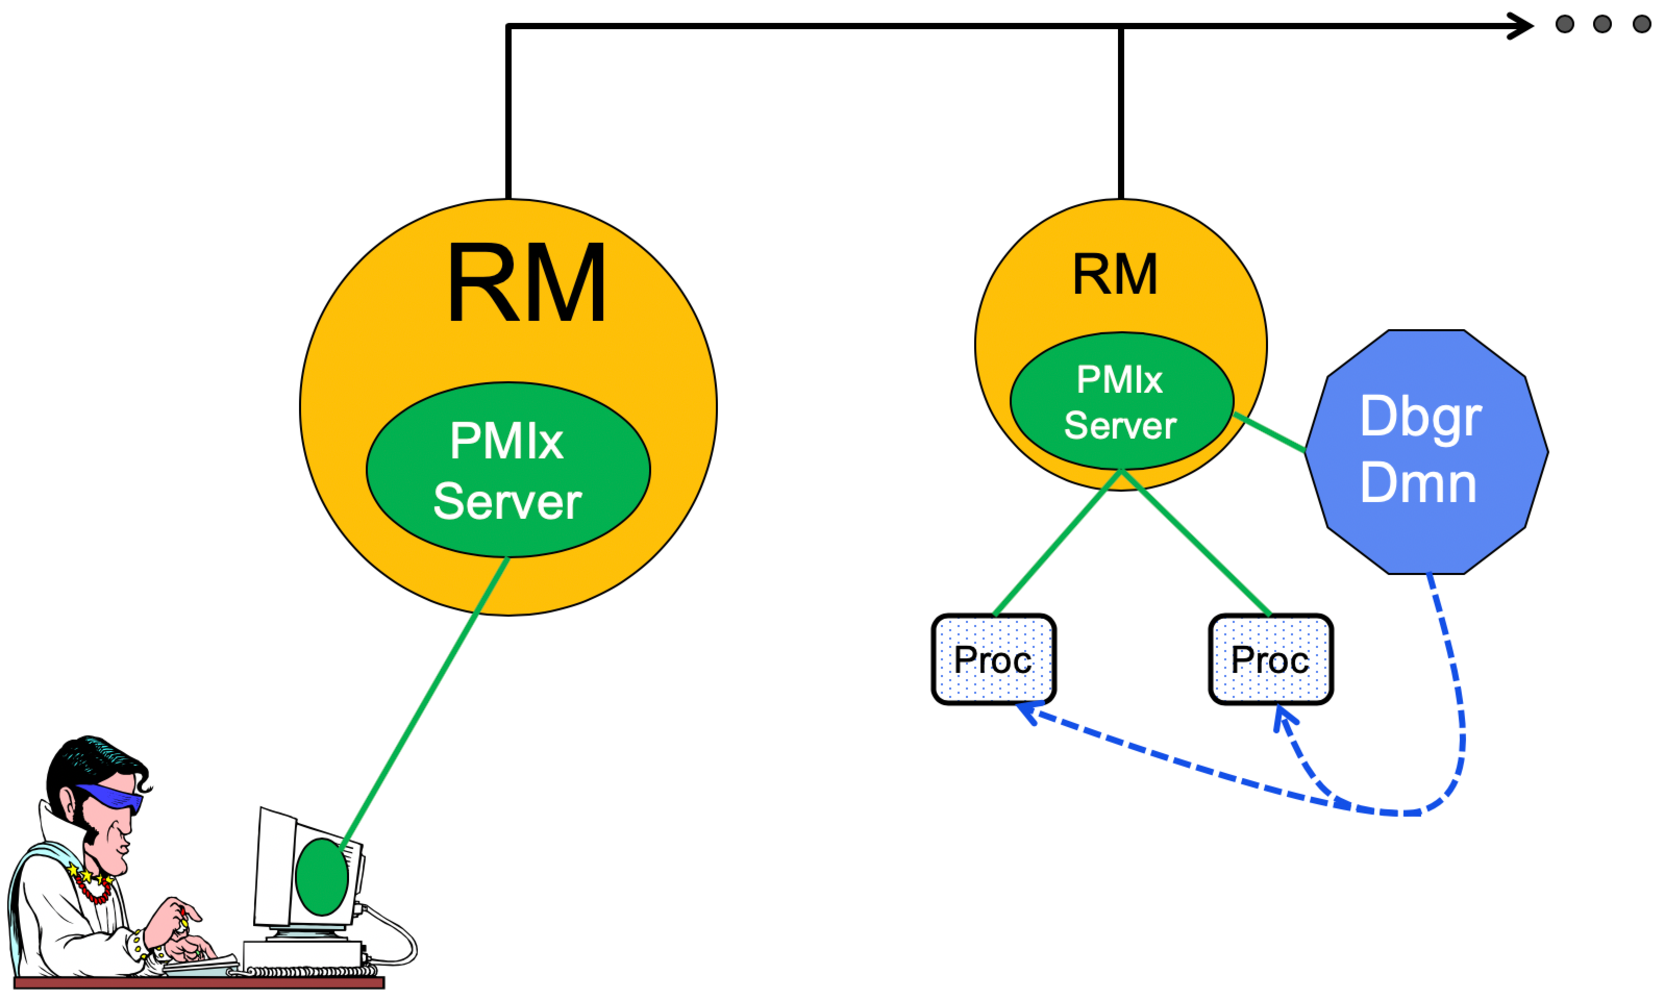
\includegraphics[clip,width=0.8\textwidth]{figs/directlaunch.pdf}
  \end{center}
  \caption{Direct Launch}
  \label{fig:dlaunch}
\end{figure*}
\endgroup


In addition to the attributes described in \refapi{PMIx_Spawn}, the tool may optionally wish to include the following tool-specific attributes in the \emph{job_info} argument to that \ac{API} (the debugger-related attributes are discussed in more detail in Section \ref{chap:api_tools:debuggers}):

\begin{itemize}
    \item \pasteAttributeItem{PMIX_FWD_STDIN}
    \item \pasteAttributeItem{PMIX_FWD_STDOUT}
    \item \pasteAttributeItem{PMIX_FWD_STDERR}
    \item \pasteAttributeItem{PMIX_FWD_STDDIAG}
    \item \pasteAttributeItem{PMIX_IOF_CACHE_SIZE}
    \item \pasteAttributeItem{PMIX_IOF_DROP_OLDEST}
    \item \pasteAttributeItem{PMIX_IOF_DROP_NEWEST}
    \item \pasteAttributeItem{PMIX_IOF_BUFFERING_SIZE}
    \item \pasteAttributeItem{PMIX_IOF_BUFFERING_TIME}
    \item \pasteAttributeItem{PMIX_IOF_TAG_OUTPUT}
    \item \pasteAttributeItem{PMIX_IOF_TIMESTAMP_OUTPUT}
    \item \pasteAttributeItem{PMIX_IOF_XML_OUTPUT}
    \item \pasteAttributeItem{PMIX_NOHUP}
    \item \pasteAttributeItem{PMIX_NOTIFY_JOB_EVENTS}
    \item \pasteAttributeItem{PMIX_NOTIFY_COMPLETION}
    \item \pasteAttributeItem{PMIX_LOG_JOB_EVENTS}
    \item \pasteAttributeItem{PMIX_DEBUG_STOP_ON_EXEC}
    \item \pasteAttributeItem{PMIX_DEBUG_STOP_IN_INIT}
    \item \pasteAttributeItem{PMIX_DEBUG_WAIT_FOR_NOTIFY}
\end{itemize}

The tool then calls the \refapi{PMIx_Spawn} \ac{API} so that the \ac{PMIx} library can communicate the spawn request to the server.

Upon receipt, the \ac{PMIx} server library passes the spawn request to its host \ac{RM} daemon for processing via the \refapi{pmix_server_spawn_fn_t} server module function. If this callback was not provided, then the \ac{PMIx} server library will return the \refconst{PMIX_ERR_NOT_SUPPORTED} error status.

If an allocation must be made, then the host environment is responsible for communicating the request to its associated scheduler. Once resources are available, the host environment initiates the launch process to start the application. The host environment must parse the spawn request for relevant directives, returning an error if any required directive cannot be supported. Optional directives may be ignored if they cannot be supported.

Any error while executing the spawn request must be returned to the requester. Once the spawn request has succeeded in starting the specified processes, the request will return \refconst{PMIX_SUCCESS} back to the requester. Upon termination of the spawned application, the host environment must generate a termination event if requested to do so - the termination event includes the status returned by the spawned application plus any other info provided by the host environment.


%%%%%%%%%%%%%%%%%%%%%%%%%%%%%%%%%%%%%%%%%%%%%%
\subsection{Indirect launch}
\label{chap:api_tools:indirect}

In the indirect launch use-case, the application processes are started via an intermediate launcher (e.g., \emph{mpiexec}) that is itself started by the tool (see Fig \ref{fig:indirlnch}). Thus, at a high level, this is a two-stage launch procedure to start the application: the tool starts the \ac{IL}, which then starts the applications. In practice, additional steps may be involved if, for example, the \ac{IL} starts its own daemons to shepherd the application processes.

A key aspect of this operational mode is the avoidance of any requirement that the tool parse and/or understand the command line of the \ac{IL}. Instead, the indirect launch support relies on \ac{PMIx} definitions to abstract the tool-launcher interaction, and on the \ac{PMIx} event notification system (Chapter \ref{chap:api_event}) to coordinate between the tool and \ac{IL}.

\adviceuserstart
The precise steps involved in starting and connecting to the \ac{IL} differ somewhat depending on whether or not an external \ac{PMIx} server (e.g., a system-level server provided by the host environment) is available. Tool developers wishing to orchestrate indirect launch themselves are referred to Section \ref{chap:api_tools:ildetail} for a detailed description of the process.
\adviceuserend

The tool spawns the \ac{IL} using the same procedure for launching an application - it assembles the description of the \ac{IL} (e.g., by parsing its command line) into a spawn request containing an array of \refstruct{pmix_app_t} and \refstruct{pmix_info_t} job-level information. An allocation of resources for the \ac{IL} itself may or may not be required – if it is, then the allocation must be made in advance or the spawn request must include allocation request information.

\begin{figure*}[ht!]
\centering
\begin{subfigure}{.5\textwidth}
  \centering
  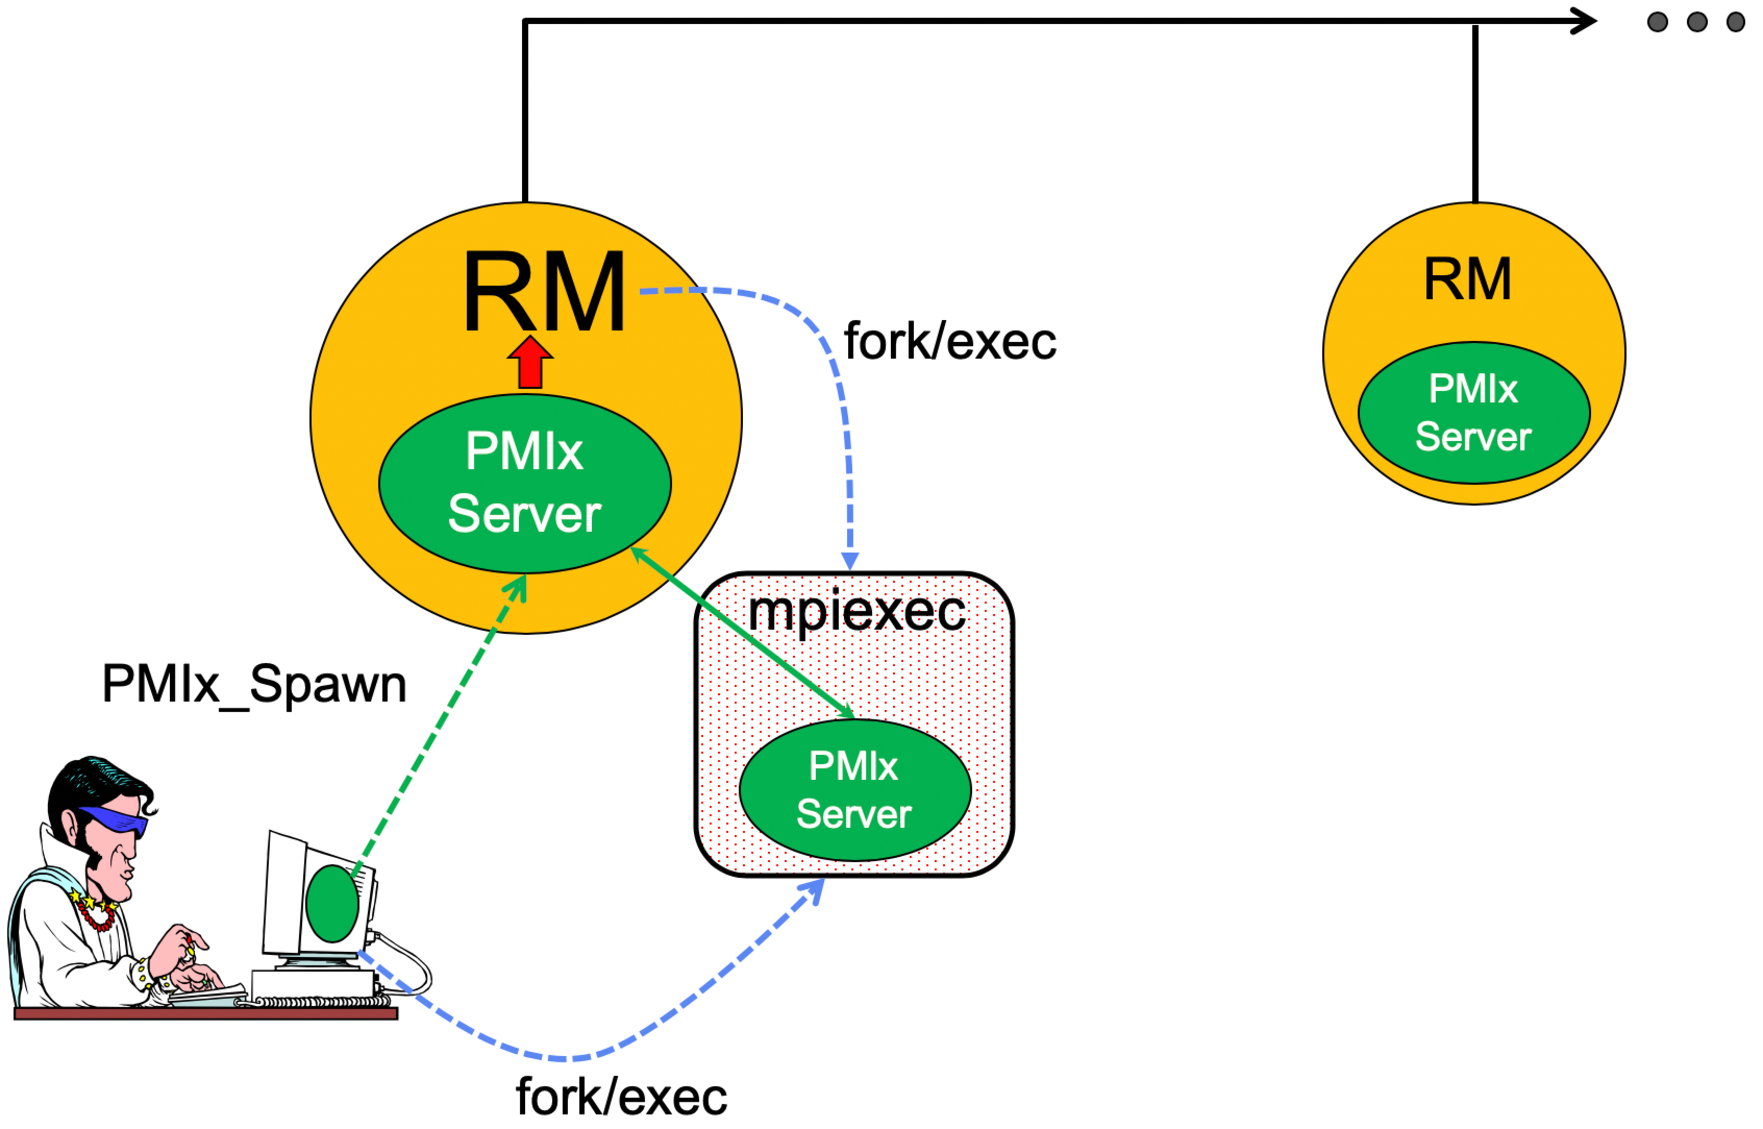
\includegraphics[width=\textwidth]{figs/indirlnch-start.pdf}
  \caption{Indirect Launch - Start}
  \label{fig:indirlnch-start}
\end{subfigure}%
\begin{subfigure}{.5\textwidth}
  \centering
  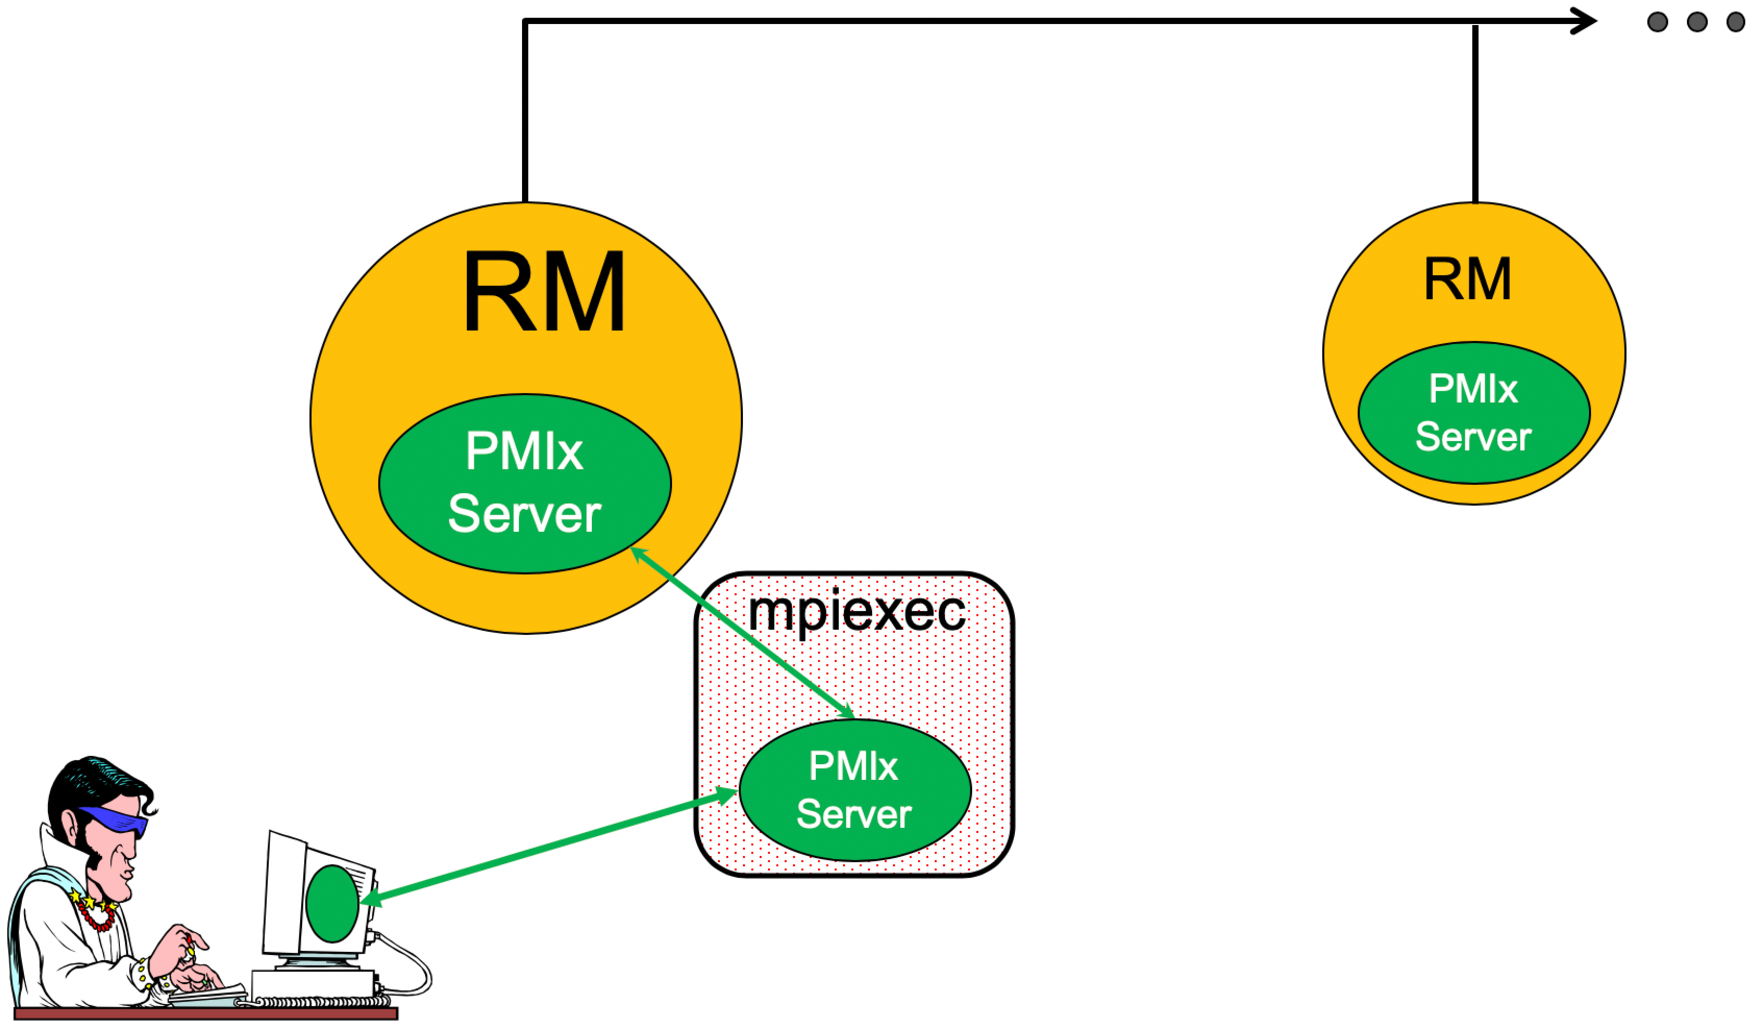
\includegraphics[width=\textwidth]{figs/indirlnch-end.pdf}
  \caption{Indirect Launch - End}
  \label{fig:indirlnch-end}
\end{subfigure}
\caption{Indirect launch procedure}
\label{fig:indirlnch}
\end{figure*}

The tool may optionally wish to include the following tool-specific attributes in the \emph{job_info} argument to \refapi{PMIx_Spawn} - note that these attributes refer to the behavior of the \ac{IL} itself and not the eventual job to be launched:

\begin{itemize}
    \item \pasteAttributeItem{PMIX_FWD_STDIN}
    \item \pasteAttributeItem{PMIX_FWD_STDOUT}
    \item \pasteAttributeItem{PMIX_FWD_STDERR}
    \item \pasteAttributeItem{PMIX_FWD_STDDIAG}
    \item \pasteAttributeItem{PMIX_IOF_CACHE_SIZE}
    \item \pasteAttributeItem{PMIX_IOF_DROP_OLDEST}
    \item \pasteAttributeItem{PMIX_IOF_DROP_NEWEST}
    \item \pasteAttributeItem{PMIX_IOF_BUFFERING_SIZE}
    \item \pasteAttributeItem{PMIX_IOF_BUFFERING_TIME}
    \item \pasteAttributeItem{PMIX_IOF_TAG_OUTPUT}
    \item \pasteAttributeItem{PMIX_IOF_TIMESTAMP_OUTPUT}
    \item \pasteAttributeItem{PMIX_IOF_XML_OUTPUT}
    \item \pasteAttributeItem{PMIX_NOHUP}
    \item \pasteAttributeItem{PMIX_LAUNCHER_DAEMON}
    \item \pasteAttributeItem{PMIX_FORKEXEC_AGENT}
    \item \pasteAttributeItem{PMIX_EXEC_AGENT}
\end{itemize}

The tool then calls the \refapi{PMIx_Spawn} \ac{API} so that the \ac{PMIx} library can either communicate the spawn request to the server (if connected to one), or locally spawn the \ac{IL} itself if not connected to a server and the \ac{PMIx} implementation includes self-spawn support. \refapi{PMIx_Spawn} shall return an error if neither of these conditions is met, or if the \ac{IL} fails to successfully complete the necessary rendezvous procedure (as detailed in Section \ref{chap:api_tools:ildetail}).

Upon successful return from \refapi{PMIx_Spawn}:

\begin{itemize}
    \item The namespace of the \ac{IL} shall be returned in the \emph{nspace} parameter of the \refapi{PMIx_Spawn} \ac{API} (or in the \refapi{pmix_spawn_cbfunc_t} for the non-blocking form of that \ac{API})
    \item The tool shall be connected to the \ac{IL} with the \ac{IL} acting as the tool's \emph{primary} server
\end{itemize}

Once \refapi{PMIx_Spawn} has returned, the tool can proceed to spawn the actual application according to the procedure describe in Section \ref{chap:api_tools:direct}.

%%%%%%%%%%%
\subsection{Tool spawn-related attributes}
\label{api:tools:attributes:spawn}

Tools are free to utilize the spawn attributes available to applications (see \ref{api:struct:attributes:spawn}) when constructing a spawn request, but can also utilize the following attributes that are specific to tool-based spawn operations:

%
\declareAttribute{PMIX_FWD_STDIN}{"pmix.fwd.stdin"}{pmix_rank_t}{
The requester intends to push information from its \code{stdin} to the indicated process. The local spawn agent should, therefore, ensure that the \code{stdin} channel to that process remains available. A rank of \refconst{PMIX_RANK_WILDCARD} indicates that all processes in the spawned job are potential recipients.
}

%
\declareAttribute{PMIX_FWD_STDOUT}{"pmix.fwd.stdout"}{bool}{
Requests that the \code{stdout} of the spawned processes be forwarded to the requester for handling
}

%
\declareAttribute{PMIX_FWD_STDERR}{"pmix.fwd.stderr"}{bool}{
Requests that the \code{stderr} of the spawned processes be forwarded to the requester for handling
}

%
\declareAttribute{PMIX_FWD_STDDIAG}{"pmix.fwd.stddiag"}{bool}{
Requests that the diagnostic channel of the spawned processes be forwarded to the requester for handling, if that channel exists
}

%
\declareNewAttribute{PMIX_NOHUP}{"pmix.nohup"}{bool}{
Any processes started on behalf of the calling tool (or the specified namespace, if such specification is included in the list of attributes) should continue after the tool disconnects from its server
}

%
\declareNewAttribute{PMIX_LAUNCHER_DAEMON}{"pmix.lnch.dmn"}{char*}{
Path to executable that is to be used as the backend daemon for the launcher. This replaces the launcher's own daemon with the specified executable. Note that the user is therefore responsible for ensuring compatibility of the specified executable and the host launcher.
}

%
\declareNewAttribute{PMIX_FORKEXEC_AGENT}{"pmix.frkex.agnt"}{char*}{
Path to executable that the launcher's backend daemons are to fork/exec in place of the actual application processes. The fork/exec agent shall connect back (as a \ac{PMIx} tool) to the launcher's daemon to receive its spawn instructions, and is responsible for starting the actual application process it replaced. See Section \ref{api:tools:debugger:agent} for details.
}

%
\declareNewAttribute{PMIX_EXEC_AGENT}{"pmix.exec.agnt"}{char*}{
Path to executable that the launcher's backend daemons are to fork/exec in place of the actual application processes. The launcher's daemon shall pass the full command line of the application on the command line of the exec agent, which shall not connect back to the launcher's daemon. The exec agent is responsible for exec'ing the specified application process in its own place. See Section \ref{api:tools:debugger:agent} for details
}


%%%%%%%%%%%
\subsection{Tool spawn-related constants}
\label{api:tools:attributes:spawnconst}

\begin{constantdesc}

%
\declareconstitemNEW{PMIX_LAUNCH_DIRECTIVE}
Launcher directives have been received from a \ac{PMIx}-enabled tool

%
\declareconstitemNEW{PMIX_LAUNCHER_READY}
Application launcher (e.g., \emph{mpiexec}) is ready to receive directives from a \ac{PMIx}-enabled tool

\end{constantdesc}

%%%%%%%%%%%%%%%%%%%%%%%%%%%%%%%%%%%%%%%%%%%%%%
%%%%%%%%%%%%%%%%%%%%%%%%%%%%%%%%%%%%%%%%%%%%%%
\section{IO Forwarding}
\label{chap:api_tools:iof}


Underlying the operation of many tools is a common need to forward \code{stdin} from the tool to targeted processes, and to return \code{stdout}/\code{stderr} from those processes to the tool (e.g., for display on the user’s console). Historically, each tool developer was responsible for creating their own \ac{IO} forwarding subsystem. However, the introduction of \ac{PMIx} as a standard mechanism for interacting between applications and the host environment has made it possible to relieve tool developers of this burden.

This section defines functions by which tools can request forwarding of input/output to/from other processes and serves as a design guide to:

\begin{itemize}
    \item provide tool developers with an overview of the expected behavior of the \ac{PMIx} \ac{IO} forwarding support;
    \item guide \ac{RM} vendors regarding roles and responsibilities expected of the \ac{RM} to support \ac{IO} forwarding; and
    \item provide insight into the thinking of the \ac{PMIx} community behind the definition of the \ac{PMIx} \ac{IO} forwarding \acp{API}
\end{itemize}

Note that the forwarding of \ac{IO} via \ac{PMIx} requires that both the host environment and the tool support \ac{PMIx}, but does not impose any similar requirements on the application itself.

The responsibility of the host environment in forwarding of \ac{IO} falls into the following areas:

\begin{itemize}
    \item Capturing output from specified processes
    \item Forwarding that output to the host of the \ac{PMIx} server library that requested it
    \item Delivering that payload to the \ac{PMIx} server library via the \refapi{PMIx_server_IOF_deliver} \ac{API} for final dispatch to the requesting tool
\end{itemize}

It is the responsibility of the \ac{PMIx} library to buffer, format, and deliver the payload to the requesting client. This may require caching of output until a forwarding registration is received, as governed by the corresponding \ac{IO} forwarding attributes of Section \ref{api:tools:attributes:iof} that are supported by the implementation.


%%%%%%%%%%%
\subsection{Forwarding stdout/stderr}

At an appropriate point in its operation (usually during startup), a tool will utilize the \refapi{PMIx_tool_init} function to connect to a \ac{PMIx} server. The \ac{PMIx} server can be hosted by an \ac{RM} daemon or could be embedded in a library-provided starter program such as \textit{mpiexec} - in terms of \ac{IO} forwarding, the operations remain the same either way. For purposes of this discussion, we will assume the server is in an \ac{RM} daemon and that the application processes are directly launched by the \ac{RM}, as shown in Fig \ref{fig:stdouterr}.

\begingroup
\begin{figure*}[ht!]
  \begin{center}
    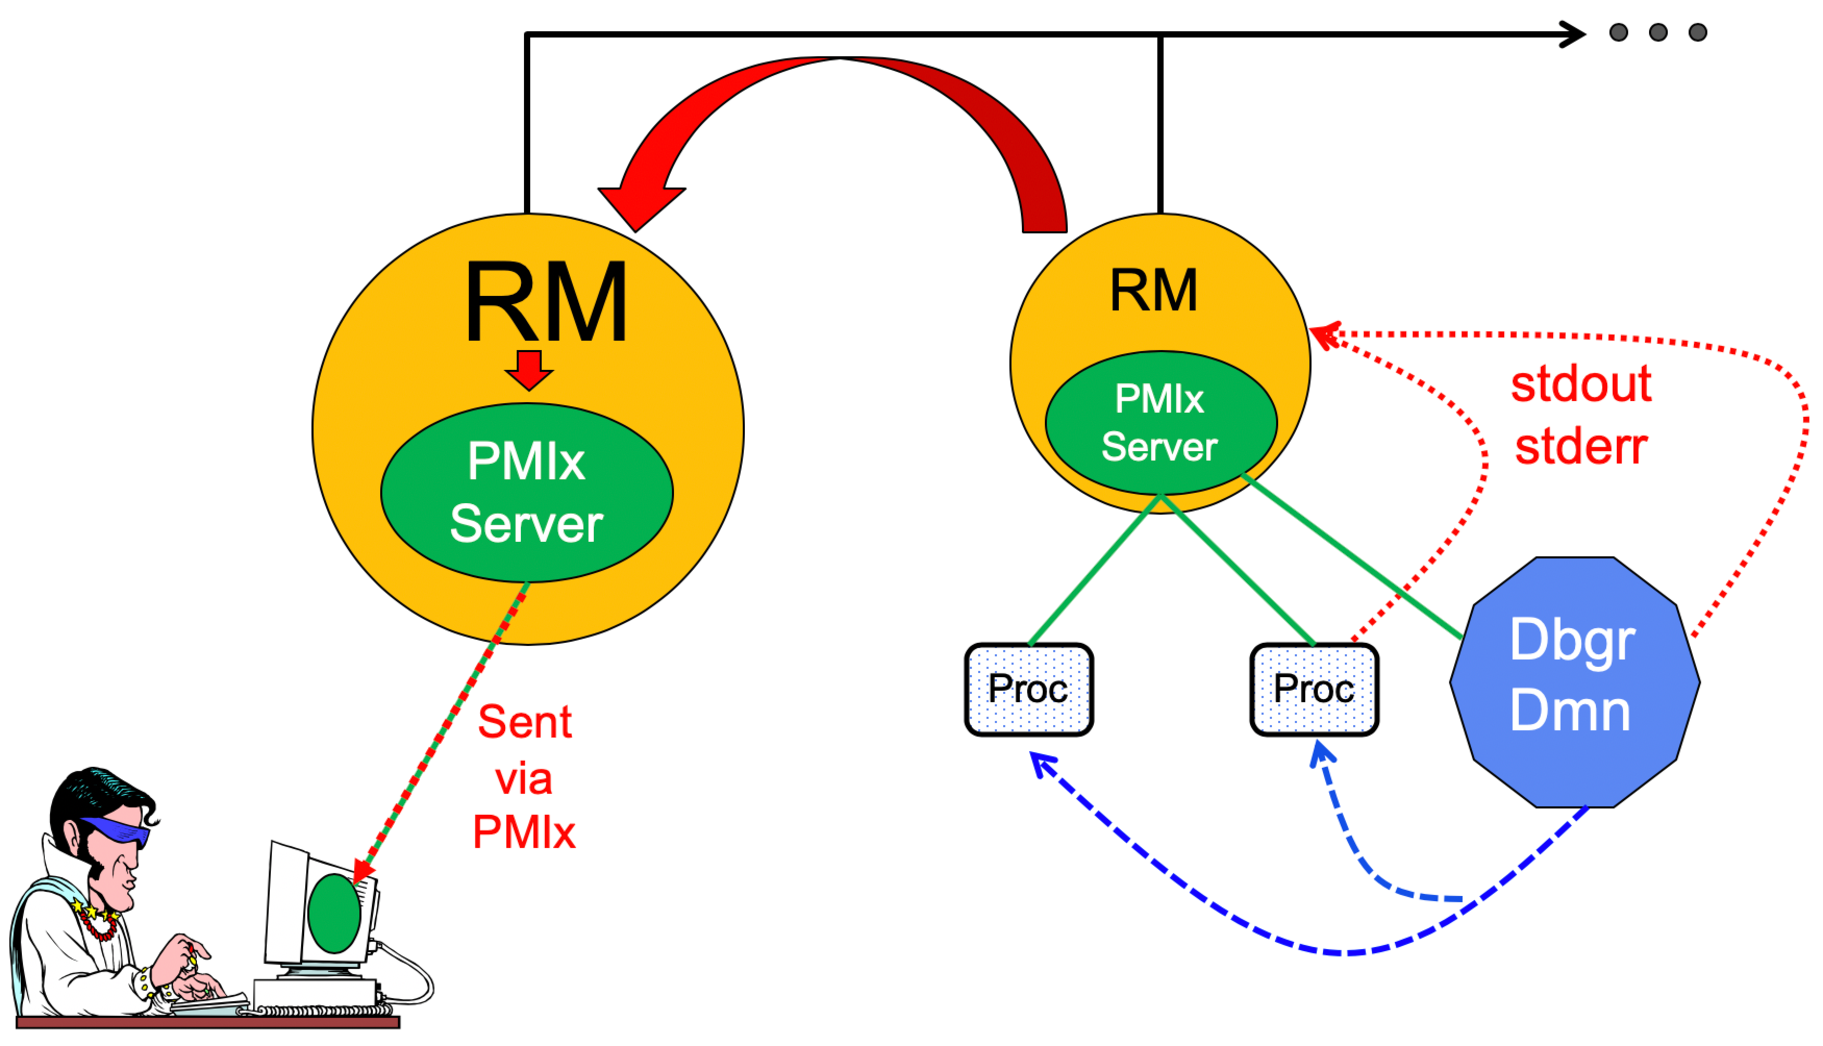
\includegraphics[clip,width=0.8\textwidth]{figs/output.pdf}
  \end{center}
  \caption{Forwarding stdout/stderr}
  \label{fig:stdouterr}
\end{figure*}
\endgroup

Once the tool has connected to the target server, it can request that processes be spawned on its behalf or that output from a specified set of existing processes in a given executing application be forwarded to it. Requests to forward output from processes being spawned by the tool should be included in calls to the \refapi{PMIx_Spawn} \ac{API} using the \refattr{PMIX_FWD_STDOUT} and/or \refattr{PMIX_FWD_STDERR} attributes. Requests to capture output from existing processes can be made via the \refapi{PMIx_IOF_pull} \ac{API}.

Two modes are supported when forwarding standard output/error:

\begin{itemize}
    \item \pasteAttributeItem{PMIX_IOF_COPY}
    \item \pasteAttributeItemBegin{PMIX_IOF_REDIRECT}This is the default mode of operation
    \pasteAttributeItemEnd{}
\end{itemize}

When requesting to forward output, the tool can specify several formatting options to be used on the resulting output stream. These include:

\begin{itemize}
    \item \pasteAttributeItem{PMIX_IOF_TAG_OUTPUT}
    \item \pasteAttributeItem{PMIX_IOF_TIMESTAMP_OUTPUT}
    \item \pasteAttributeItem{PMIX_IOF_XML_OUTPUT}
\end{itemize}

The \ac{PMIx} client in the tool is responsible for formatting the output stream. Note that output from multiple processes will often be interleaved due to variations in arrival time - ordering of output is not guaranteed across processes and/or nodes.

%%%%%%%%%%%
\subsection{Forwarding stdin}

A tool is not necessarily a child of the \ac{RM} as it may have been started directly from the command line. Thus, provision must be made for the tool to collect its \code{stdin} and pass it to the host \ac{RM} (via the \ac{PMIx} server) for forwarding. Two methods of support for forwarding of \code{stdin} are defined:

\begingroup
\begin{figure*}[ht!]
  \begin{center}
    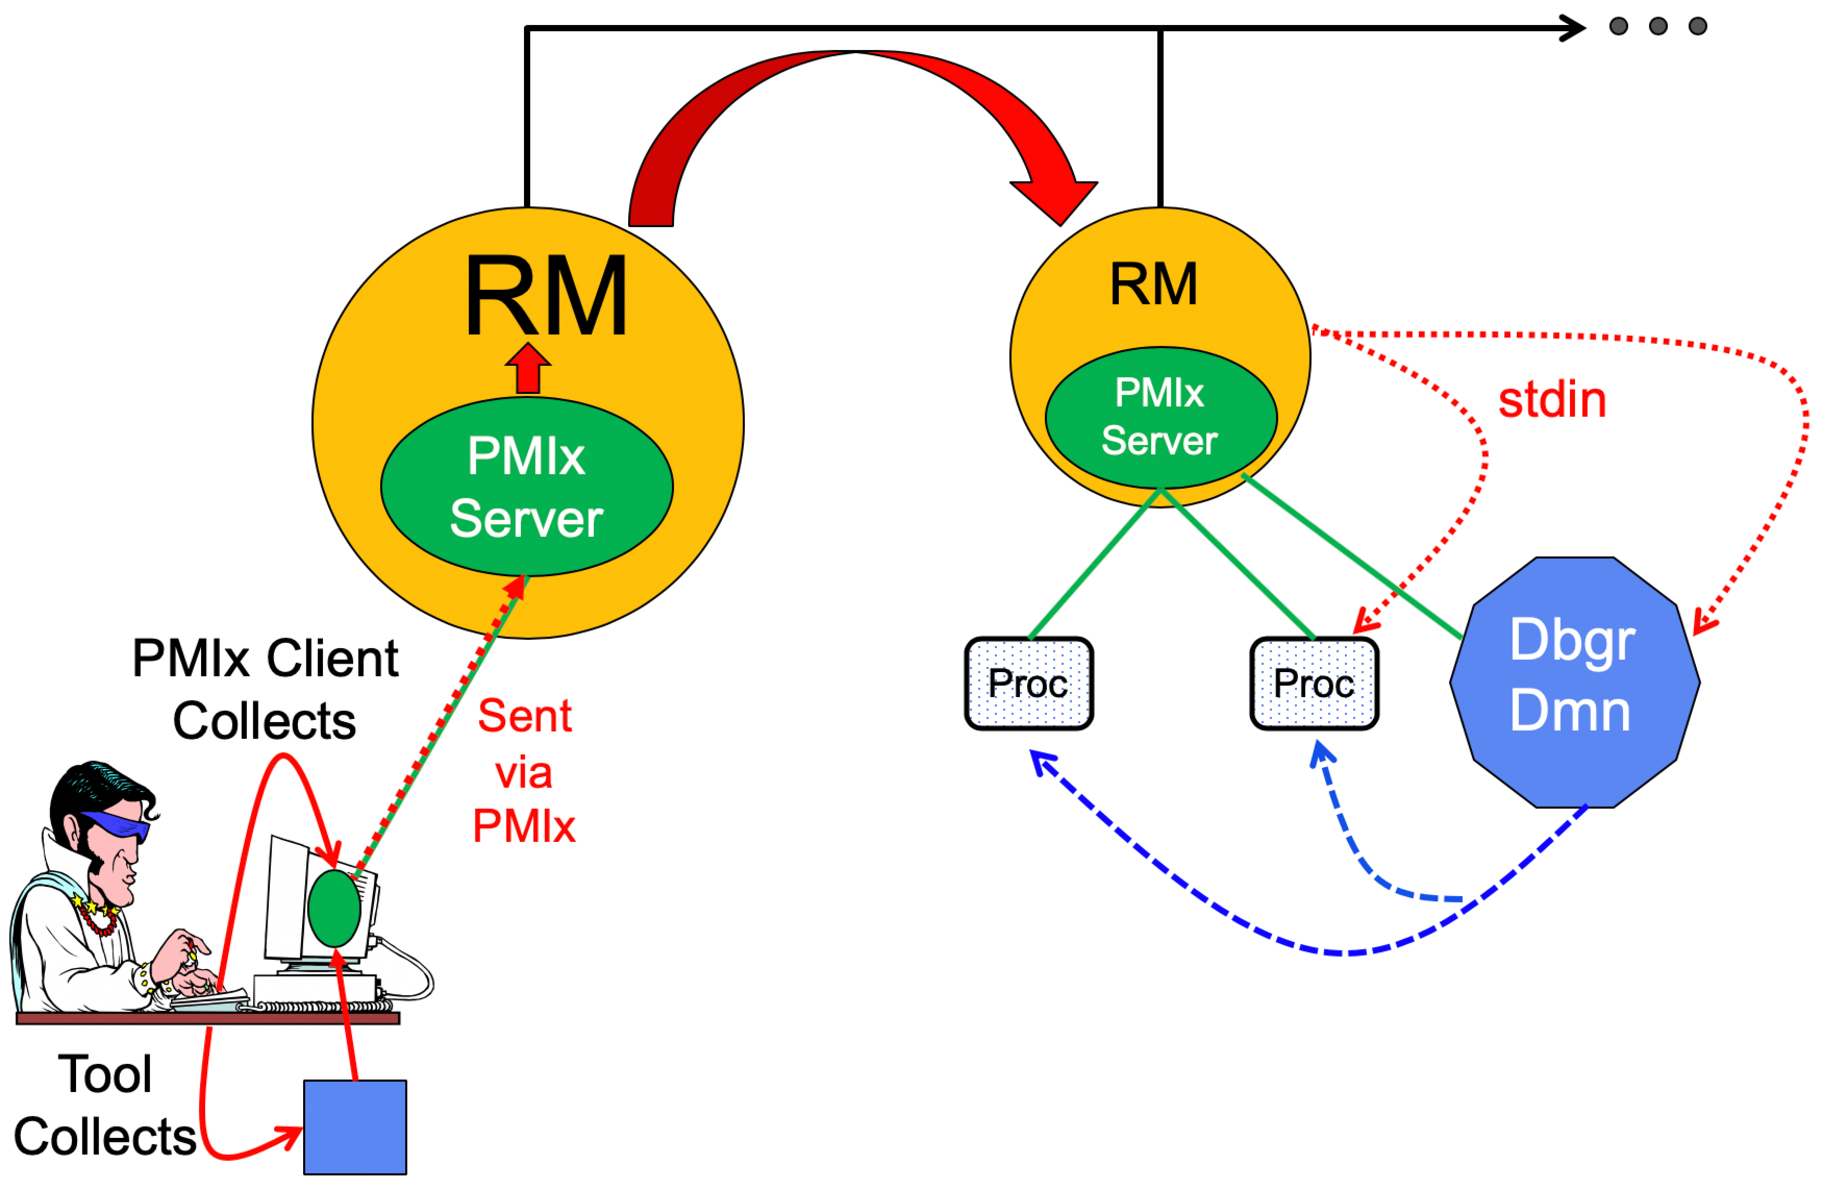
\includegraphics[clip,width=0.8\textwidth]{figs/stdin.pdf}
  \end{center}
  \caption{Forwarding stdin}
  \label{fig:stdin}
\end{figure*}
\endgroup

\begin{itemize}
    \item internal collection by the \ac{PMIx} tool library itself. This is requested via the \refattr{PMIX_IOF_PUSH_STDIN} attribute in the \refapi{PMIx_IOF_push} call. When this mode is selected, the tool library begins collecting all \code{stdin} data and internally passing it to the local server for distribution to the specified target processes. All collected data is sent to the same targets until \code{stdin} is closed, or a subsequent call to \refapi{PMIx_IOF_push} is made that includes the \refattr{PMIX_IOF_COMPLETE} attribute indicating that forwarding of \code{stdin} is to be terminated.
    \item external collection directly by the tool. It is assumed that the tool will provide its own code/mechanism for collecting its \code{stdin} as the tool developers may choose to insert some filtering and/or editing of the stream prior to forwarding it. In addition, the tool can directly control the targets for the data on a per-call basis – i.e., each call to \refapi{PMIx_IOF_push} can specify its own set of target recipients for that particular \emph{blob} of data. Thus, this method provides maximum flexibility, but requires that the tool developer provide their own code to capture \code{stdin}.
\end{itemize}

Note that it is the responsibility of the \ac{RM} to forward data to the host where the target process(es) are executing, and for the host daemon on that node to deliver the data to the \code{stdin} of target process(es).. The \ac{PMIx} server on the remote node is not involved in this process. Systems that do not support forwarding of \code{stdin} shall return \refconst{PMIX_ERR_NOT_SUPPORTED} in response to a forwarding request.

\adviceuserstart
Scalable forwarding of \code{stdin} represents a significant challenge. Most environments will at least handle a \emph{send-to-1} model whereby \code{stdin} is forwarded to a single identified process, and occasionally an additional \emph{send-to-all} model where \code{stdin} is forwarded to all processes in the application. Users are advised to check their host environment for available support as the distribution method lies outside the scope of \ac{PMIx}.

\code{Stdin} buffering by the \ac{RM} and/or \ac{PMIx} library can be problematic. If any targeted recipient is slow reading data (or decides never to read data), then the data must be buffered in some intermediate daemon or the \ac{PMIx} tool library itself. Thus, piping a large amount of data into \code{stdin} can result in a very large memory footprint in the system management stack or the tool. Best practices, therefore, typically focus on reading of input files by application processes as opposed to forwarding of \code{stdin}.
\adviceuserend


%%%%%%%%%%%
\subsection{IO Forwarding attributes}
\label{api:tools:attributes:iof}

The following attributes are used to control \ac{IO} forwarding behavior at the request of tools.

%
\declareAttribute{PMIX_IOF_CACHE_SIZE}{"pmix.iof.csize"}{uint32_t}{
The requested size of the \ac{PMIx} server cache in bytes for each specified channel. By default, the server is allowed (but not required) to drop all bytes received beyond the max size.
}

%
\declareAttribute{PMIX_IOF_DROP_OLDEST}{"pmix.iof.old"}{bool}{
In an overflow situation, the \ac{PMIx} server is to drop the oldest bytes to make room in the cache.
}

%
\declareAttribute{PMIX_IOF_DROP_NEWEST}{"pmix.iof.new"}{bool}{
In an overflow situation, the \ac{PMIx} server is to drop any new bytes received until room becomes available in the cache (default).
}

%
\declareAttribute{PMIX_IOF_BUFFERING_SIZE}{"pmix.iof.bsize"}{uint32_t}{
Requests that \ac{IO} on the specified channel(s) be aggregated in the \ac{PMIx} tool library until the specified number of bytes is collected to avoid being called every time a block of \ac{IO} arrives. The \ac{PMIx} tool library will execute the callback and reset the collection counter whenever the specified number of bytes becomes available. Any remaining buffered data will be \emph{flushed} to the callback upon a call to deregister the respective channel.
}

%
\declareAttribute{PMIX_IOF_BUFFERING_TIME}{"pmix.iof.btime"}{uint32_t}{
Max time in seconds to buffer \ac{IO} before delivering it. Used in conjunction with buffering size, this prevents \ac{IO} from being held indefinitely while waiting for another payload to arrive.
}

%
\declareAttribute{PMIX_IOF_COMPLETE}{"pmix.iof.cmp"}{bool}{
Indicates that the specified \ac{IO} channel has been closed by the source.
}

%
\declareAttribute{PMIX_IOF_TAG_OUTPUT}{"pmix.iof.tag"}{bool}{
Requests that output be prefixed with the nspace,rank of the source and a string identifying the channel (\code{stdout}, \code{stderr}, etc.)
}

%
\declareAttribute{PMIX_IOF_TIMESTAMP_OUTPUT}{"pmix.iof.ts"}{bool}{
Requests that output be marked with the time at which the data was received by the tool - note that this will differ from the time at which the data was collected from the source
}

%
\declareAttribute{PMIX_IOF_XML_OUTPUT}{"pmix.iof.xml"}{bool}{
Requests that output be formatted in \ac{XML}
}

\declareNewAttribute{PMIX_IOF_PUSH_STDIN}{"pmix.iof.stdin"}{bool}{
Requests that the \ac{PMIx} library collect the \code{stdin} of the requester and forward it to the processes specified in the \refapi{PMIx_IOF_push} call. All collected data is sent to the same targets until \code{stdin} is closed, or a subsequent call to \refapi{PMIx_IOF_push} is made that includes the \refattr{PMIX_IOF_COMPLETE} attribute indicating that forwarding of \code{stdin} is to be terminated.
}

\declareNewAttribute{PMIX_IOF_COPY}{"pmix.iof.cpy"}{bool}{
Requests that the host environment deliver a copy of the specified output stream(s) to the tool, letting the stream(s) continue to also be delivered to the default location. This allows the tool to tap into the output stream(s) without redirecting it from its current final destination
}

\declareNewAttribute{PMIX_IOF_REDIRECT}{"pmix.iof.redir"}{bool}{
Requests that the host environment intercept the specified output stream(s) and deliver it to the requesting tool instead of its current final destination. This might be used, for example, during a debugging procedure to avoid injection of debugger-related output into the application’s results file. The original output stream(s) destination is restored upon termination of the tool
}

%%%%%%%%%%%%%%%%%%%%%%%%%%%%%%%%%%%%%%%%%%%%%%
%%%%%%%%%%%%%%%%%%%%%%%%%%%%%%%%%%%%%%%%%%%%%%
\section{Debugger Support}
\label{chap:api_tools:debuggers}

Debuggers are a class of tool that merits special consideration due to their particular requirements for access to job-related information and control over process execution. The primary advantage of using \ac{PMIx} for these purposes lies in the resulting portability of the debugger as it can be used with any system and/or programming model that supports \ac{PMIx}. In addition to the general tool support described above, debugger support includes:

\begin{itemize}
    \item Co-location, co-spawn, and communication wireup of debugger daemons for scalable launch. This includes providing debugger daemons with endpoint connection information across the daemons themselves.
    \item Identification of the job that is to be debugged. This includes automatically providing debugger daemons with the job-level information for their target job
\end{itemize}

Debuggers can also utilize the options in the \refapi{PMIx_Spawn} \ac{API} to exercise a degree of control over spawned jobs for debugging purposes. For example, a debugger can utilize the environmental parameter attributes of Section \ref{api:struct:attributes:envar} to request \code{LD_PRELOAD} of a memory interceptor library prior to spawning an application process, or interject a custom fork/exec agent to shepherd the application process.

A key element of the debugging process is the ability of the debugger to require that processes \emph{pause} at some well-defined point, thereby providing the debugger with an opportunity to attach and control execution. The actual implementation of the \emph{pause} lies outside the scope of \ac{PMIx} - it typically requires either the launcher or the application itself to implement the necessary operations. However, \ac{PMIx} does provide several standard attributes by which the debugger can specify the desired attach point:

\begin{itemize}
    \item \pasteAttributeItemBegin{PMIX_DEBUG_STOP_ON_EXEC}Launchers that cannot support this operation shall return an error from the \refapi{PMIx_Spawn} \ac{API} if this behavior is requested.
    \pasteAttributeItemEnd{}
    \item \pasteAttributeItemBegin{PMIX_DEBUG_STOP_IN_INIT}\ac{PMIx} implementations that do not support this operation shall return an error from \refapi{PMIx_Init} if this behavior is requested. Launchers that cannot support this operation shall return an error from the \refapi{PMIx_Spawn} \ac{API} if this behavior is requested.
    \pasteAttributeItemEnd{}
    \item \pasteAttributeItemBegin{PMIX_DEBUG_WAIT_FOR_NOTIFY}Launchers that cannot support this operation shall return an error from the \refapi{PMIx_Spawn} \ac{API} if this behavior is requested.
    \pasteAttributeItemEnd{}
\end{itemize}

Note that there is no mechanism by which the \ac{PMIx} library or the launcher can verify that an application will recognize and support the \refattr{PMIX_DEBUG_WAIT_FOR_NOTIFY} request. Debuggers utilizing this attachment method must, therefore, be prepared to deal with the case where the application fails to recognize and/or honor the request.

If the \ac{PMIx} implementation and/or the host environment support it, debuggers can utilize the \refapi{PMIx_Query_info} \ac{API} to determine which features are available via the \refattr{PMIX_QUERY_ATTRIBUTE_SUPPORT} attribute:

\begin{itemize}
    \item \refattr{PMIX_DEBUG_STOP_IN_INIT} by checking \refattr{PMIX_CLIENT_ATTRIBUTES} for the \refapi{PMIx_Init} \ac{API}
    \item \refattr{PMIX_DEBUG_STOP_ON_EXEC} by checking \refattr{PMIX_HOST_ATTRIBUTES} for the \refapi{PMIx_Spawn} \ac{API}
\end{itemize}

The target namespace or process (as given by the debugger in the spawn request) shall be provided to each daemon in its job-level information via the \refattr{PMIX_DEBUG_TARGET} attribute. Debugger daemons are responsible for self-determining their specific target process(es), and can then utilize the \refapi{PMIx_Query_info} \ac{API} to obtain information about them (see Fig \ref{fig:dbgptable}) - e.g., to obtain the \acp{PID} of the local processes to which they need to attach. \ac{PMIx} provides the \refstruct{pmix_proc_info_t} structure for organizing information about a process' \ac{PID}, location, and state. Debuggers may request information on a given job at two levels:

\begin{itemize}
    \item \pasteAttributeItem{PMIX_QUERY_PROC_TABLE}
    \item \pasteAttributeItem{PMIX_QUERY_LOCAL_PROC_TABLE}
\end{itemize}

Note that the information provided in the returned proctable represents a snapshot in time.

\begingroup
\begin{figure*}[ht!]
  \begin{center}
    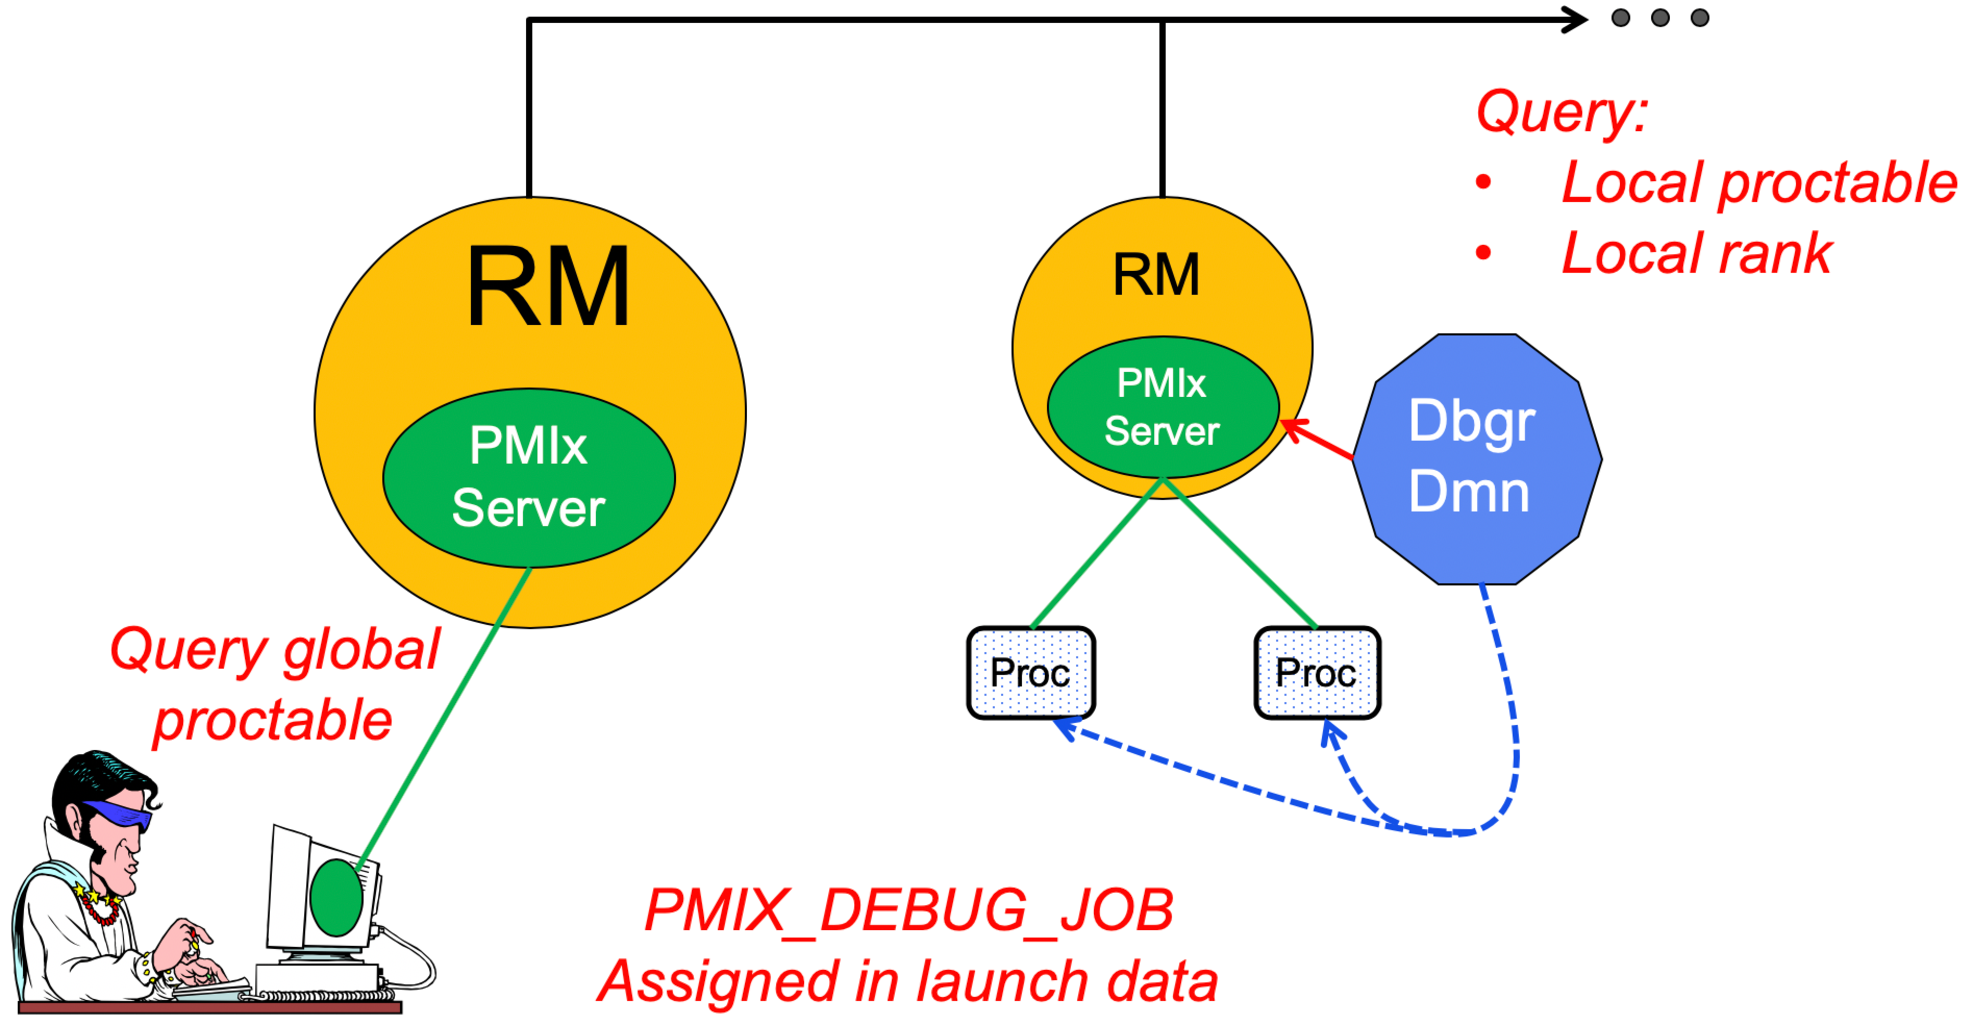
\includegraphics[clip,width=0.8\textwidth]{figs/dbgptable.pdf}
  \end{center}
  \caption{Obtaining proctables}
  \label{fig:dbgptable}
\end{figure*}
\endgroup

Debugger daemons can be started in two ways - either at the same time the application is spawned, or separately at a later time.

%%%%%%%%%%%%%%%%%%%%%%%%%%%%%%%%%%%%%%%%%%%%%%
\subsection{Co-Location of Debugger Daemons}
\label{chap:api_tools:colocate}

Debugging operations typically require the use of daemons that are located on the same node as the processes they are attempting to debug. The debugger can, of course, specify its own mapping method when issuing its spawn request or utilize its own internal launcher to place the daemons. However, when attaching to a running job, \ac{PMIx} provides debuggers with a simplified method for requesting that the launcher associated with the job \emph{co-locate} the required daemons. Debuggers can request \emph{co-location} of their daemons by adding the following attributes to the \refapi{PMIx_Spawn} used to spawn them:

\begin{itemize}
    \item \refattr{PMIX_DEBUGGER_DAEMONS} - indicating that the launcher is being asked to spawn debugger daemons
    \item \refattr{PMIX_DEBUG_TARGET} - indicating the job or process that is to be debugged. This allows the launcher to identify the processes to be debugged and their location.
    \item \refattr{PMIX_DEBUG_DAEMONS_PER_PROC} - specifies the number of debugger daemons to be co-located per target process.
    \item \refattr{PMIX_DEBUG_DAEMONS_PER_NODE} - specifies the number of debugger daemons to be co-located per node where at least one target process is executing.
\end{itemize}

Debugger daemons spawned in this manner shall be provided with the typical \ac{PMIx} information for their own job, plus the target they are to debug via the \refattr{PMIX_DEBUG_TARGET} attribute. The debugger daemons spawned on a given node are responsible for self-determining their specific target process(es). Note that this method for starting the debugger precludes the use of \ac{PMIx} attributes to \emph{pause} the application prior to attaching the debugger. Users are referred to the \refapi{PMIx_Job_control} \ac{API} for possible alternative methods.


%%%%%%%%%%%%%%%%%%%%%%%%%%%%%%%%%%%%%%%%%%%%%%
\subsection{Co-Spawn of Debugger Daemons}
\label{chap:api_tools:cospawn}

In the case where a job is being spawned under the control of a debugger, \ac{PMIx} provides a shortcut method for spawning the debugger's daemons in parallel with the job. This requires that the debugger be specified as one of the \refstruct{pmix_app_t} in the same spawn command used to start the job. The debugger application must include at least the \refattr{PMIX_DEBUGGER_DAEMONS} attribute identifying itself as a debugger, and may utilize either a mapping option to direct daemon placement, or one of the \refattr{PMIX_DEBUG_DAEMONS_PER_PROC} or \refattr{PMIX_DEBUG_DAEMONS_PER_NODE} directives.

The launcher is not to include the debugger daemons in the job-level info provided to the rest of the \refstruct{pmix_app_t}s, nor in any calculated rank values (e.g., PMIX_NODE_RANK or PMIX_LOCAL_RANK) in those applications. The launcher is free to implement the launch as a single operation for both the applications and debugger daemons (preferred), or may stage the launches as required. The launcher shall not return from the \refapi{PMIx_Spawn} command until all included applications and the debugger daemons have been started.

%%%%%%%%%%%%%%%%%%%%%%%%%%%%%%%%%%%%%%%%%%%%%%
\subsection{Debugger Agents}
\label{api:tools:debugger:agent}

Individual debuggers may, depending upon implementation, require varying degrees of control over each application process when it is started beyond those available via directives to \refapi{PMIx_Spawn}. \ac{PMIx} offers two mechanisms to help provide a means of meeting these needs.

The \refattr{PMIX_FORKEXEC_AGENT} attribute allows the debugger to specify an intermediate process (the \ac{FEA}) for spawning the actual application process (see Fig. \ref{fig:dbgfea}), thereby interposing the debugger daemon between the application process and the launcher's daemon. Instead of spawning the application process, the launcher will spawn the \ac{FEA}, which will connect back to the \ac{PMIx} server as a tool to obtain the spawn description of the application process it is to spawn. The \ac{PMIx} server in the launcher's daemon shall not register the fork/exec agent as a local client process, nor shall the launcher include the agent in any of the job-level values (e.g., \refattr{PMIX_RANK} within the job or \refattr{PMIX_LOCAL_RANK} on the node) provided to the application process. The launcher shall treat the collection of \acp{FEA} as a debugger job equivalent to the co-spawn use-case described in Section \ref{chap:api_tools:cospawn}.

\begin{figure*}[ht!]
\centering
\begin{subfigure}{.5\textwidth}
  \centering
  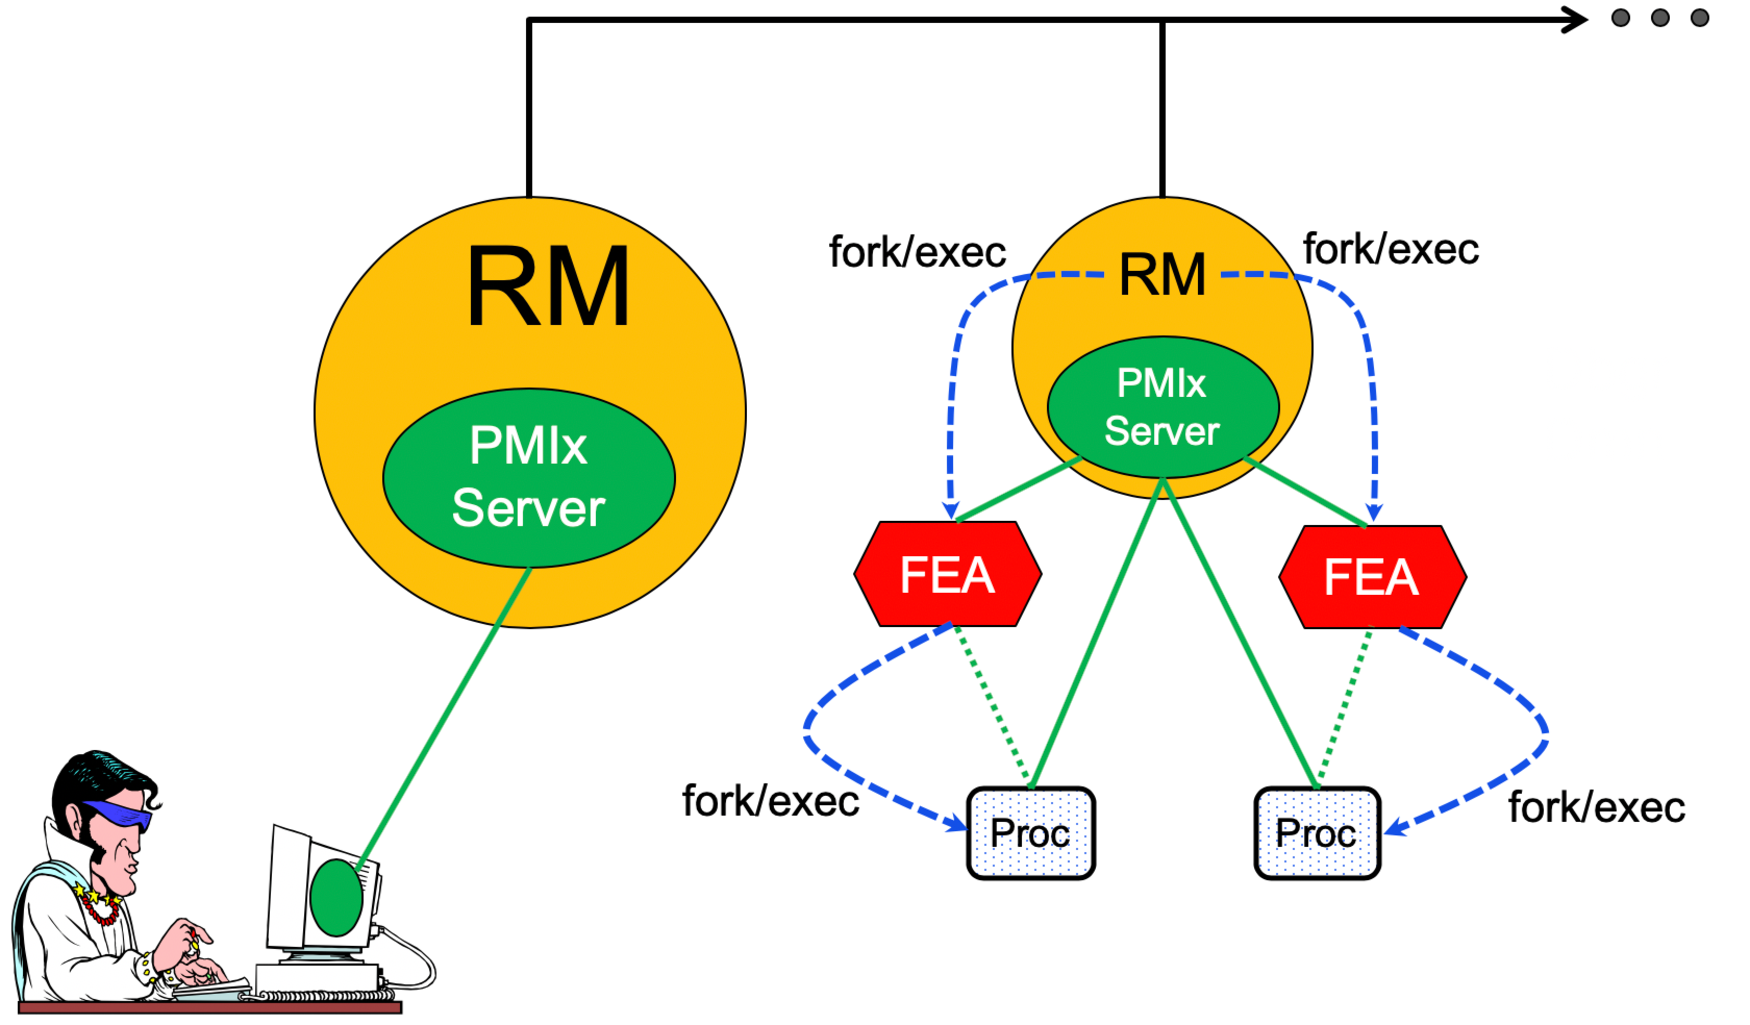
\includegraphics[width=\textwidth]{figs/dbgfea.pdf}
  \caption{Fork/exec agent}
  \label{fig:dbgfea}
\end{subfigure}%
\begin{subfigure}{.5\textwidth}
  \centering
  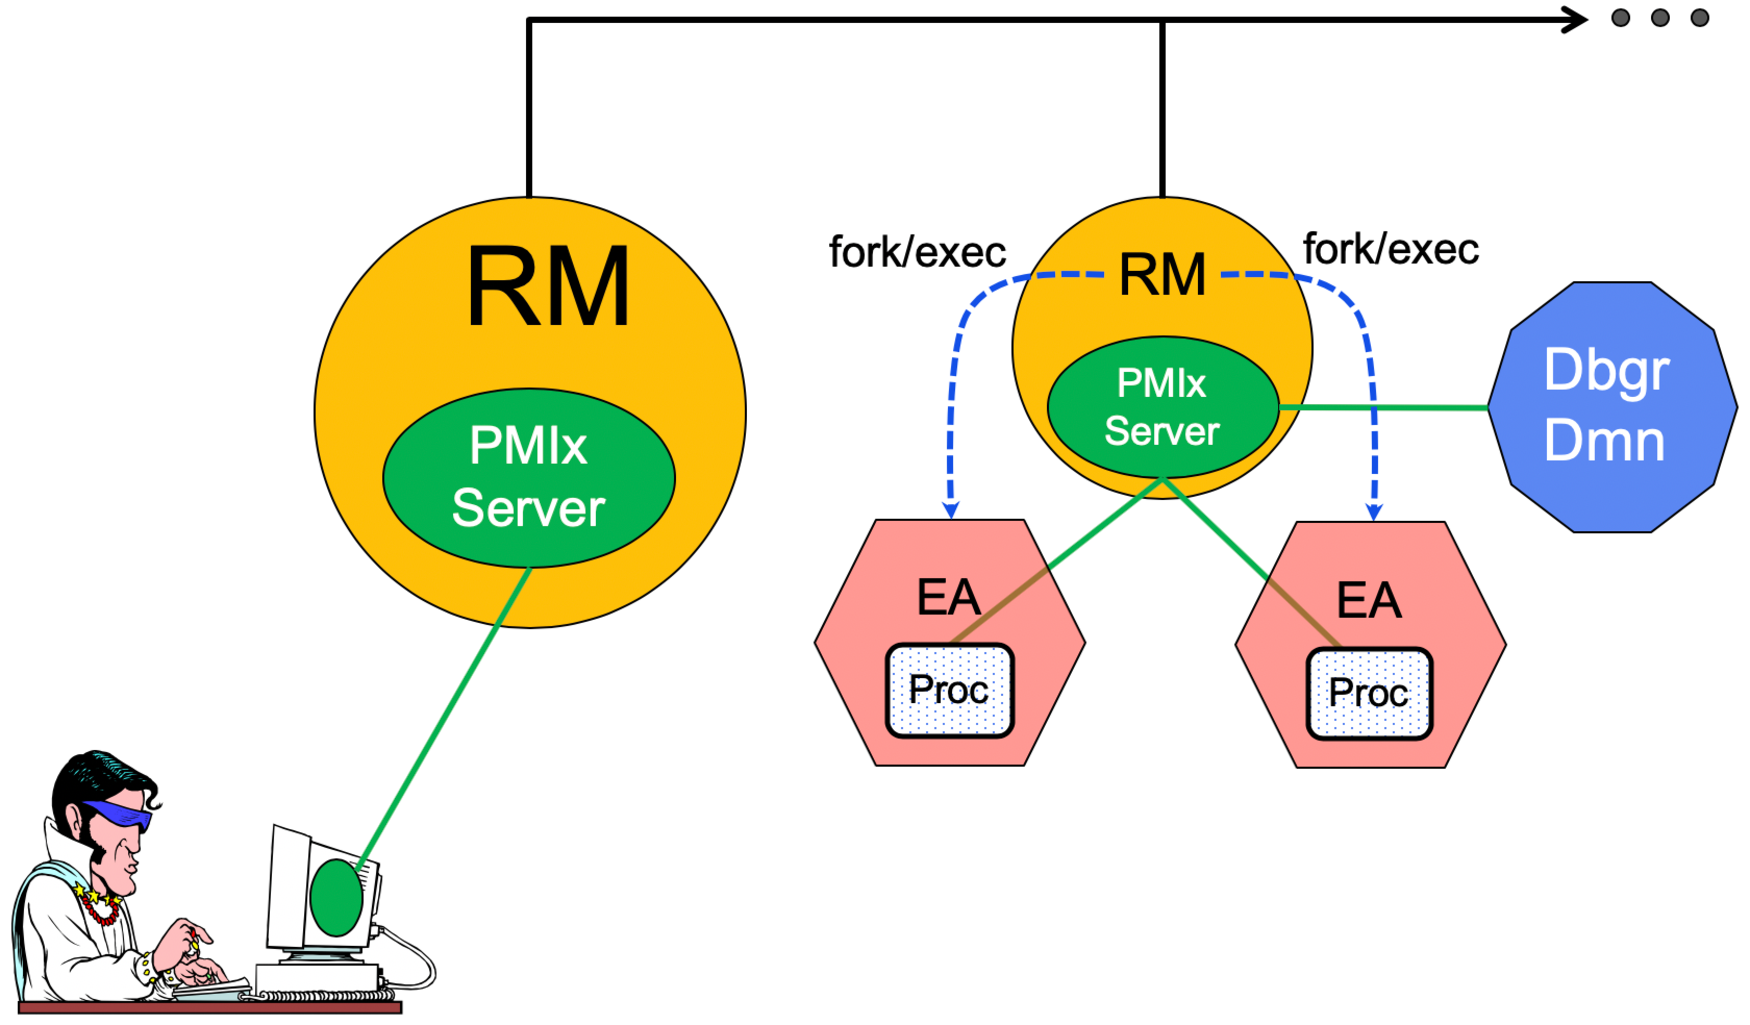
\includegraphics[width=\textwidth]{figs/dbgea.pdf}
  \caption{Exec agent}
  \label{fig:dbgea}
\end{subfigure}
\caption{Intermediate agents}
\label{fig:dbginta}
\end{figure*}

In contrast, the \refattr{PMIX_EXEC_AGENT} attribute (Fig. \ref{fig:dbgea}) allows the debugger to specify an agent that will perform some preparatory actions and then exec the eventual application process to replace itself. In this scenario, the exec agent is provided with the application process' command line as arguments on its command line (e.g., "./agent appargv[0] appargv[1]") and does not connect back to the host's \ac{PMIx} server. It is the responsibility of the exec agent to properly separate its own command line arguments (if any) from the application description.

%%%%%%%%%%%
\subsection{Debugger-related constants}
\label{api:tools:attributes:dbgconst}

\begin{constantdesc}

%
\declareconstitemNEW{PMIX_DEBUG_WAITING_FOR_NOTIFY}
Job to be debugged is waiting for a release - this is not a value accessed using the \refapi{PMIx_Get} \ac{API}.


\declareconstitemNEW{PMIX_DEBUGGER_RELEASE}
Release processes that are paused awaiting debugger attach

%
\declareconstitemDEP{PMIX_ERR_DEBUGGER_RELEASE}
Error in debugger release - deprecated in favor of \refconst{PMIX_DEBUGGER_RELEASE}

\end{constantdesc}

%%%%%%%%%%%
\subsection{Debugger attributes}
\label{api:struct:attributes:debugger}

Attributes used to assist debuggers - these are values that can either be passed to the \refapi{PMIx_Spawn} \acp{API} or accessed by a debugger itself using the \refapi{PMIx_Get} \ac{API} with the \refconst{PMIX_RANK_WILDCARD} rank.

%
\declareAttribute{PMIX_DEBUG_STOP_ON_EXEC}{"pmix.dbg.exec"}{bool}{
Included in either the \emph{pmix_info_t} array in a \refstruct{pmix_app_t} description (if the directive applies only to that application) or in the \emph{job_info} array if it applies to all applications in the given spawn request. Indicates that the application is being spawned under a debugger, and that the local launch agent is to pause the resulting application processes on first instruction for debugger attach. The launcher (\ac{RM} or \ac{IL}) is to generate the \refconst{PMIX_LAUNCH_COMPLETE} event when all processes are stopped at the exec point.
}

%
\declareAttribute{PMIX_DEBUG_STOP_IN_INIT}{"pmix.dbg.init"}{bool}{
Included in either the \emph{pmix_info_t} array in a \refstruct{pmix_app_t} description (if the directive applies only to that application) or in the \emph{job_info} array if it applies to all applications in the given spawn request. Indicates that the specified application is being spawned under a debugger. The \ac{PMIx} client library in each resulting application process shall notify its \ac{PMIx} server that it is pausing and then pause during \refapi{PMIx_Init} of the spawned processes until receipt of the \refconst{PMIX_DEBUGGER_RELEASE} event. The launcher (\ac{RM} or \ac{IL}) is responsible for generating the \refconst{PMIX_DEBUG_WAITING_FOR_NOTIFY} event when all processes have reached the pause point.
}

%
\declareAttribute{PMIX_DEBUG_WAIT_FOR_NOTIFY}{"pmix.dbg.notify"}{bool}{
Included in either the \emph{pmix_info_t} array in a \refstruct{pmix_app_t} description (if the directive applies only to that application) or in the \emph{job_info} array if it applies to all applications in the given spawn request. Indicates that the specified application is being spawned under a debugger. The resulting application processes are to notify their server when they reach some application-determined location and pause at that point until receipt of the \refconst{PMIX_DEBUGGER_RELEASE} event. The launcher (\ac{RM} or \ac{IL}) is responsible for generating the \refconst{PMIX_DEBUG_WAITING_FOR_NOTIFY} event when all processes have indicated they are at the pause point.
}

%
\declareDepAttribute{PMIX_DEBUG_JOB}{"pmix.dbg.job"}{char*}{
Namespace of the job to be debugged - provided to the debugger upon launch (replaced by \refattr{PMIX_DEBUG_TARGET})
}

%
\declareNewAttribute{PMIX_DEBUG_TARGET}{"pmix.dbg.tgt"}{pmix_proc_t*}{
Identifier of process(es) to be debugged - a rank of \refconst{PMIX_RANK_WILDCARD} indicates that all processes in the specified namespace are to be included
}

%
\declareAttribute{PMIX_DEBUGGER_DAEMONS}{"pmix.debugger"}{bool}{
Included in the \emph{info} array of a \refstruct{pmix_app_t}, this attribute declares that the application consists of debugger daemons and shall be governed accordingly. If used as the sole \refstruct{pmix_app_t} in a \refapi{PMIx_Spawn} request, then the \refattr{PMIX_DEBUG_TARGET} attribute must also be provided (in either the \emph{job_info} or in the \emph{info} array of the \refstruct{pmix_app_t}) to identify the namespace to be debugged so that the launcher can determine where to place the spawned daemons. If neither \refattr{PMIX_DEBUG_DAEMONS_PER_PROC} nor \refattr{PMIX_DEBUG_DAEMONS_PER_NODE} is specified, then the launcher shall default to a placement policy of one daemon per process in the target job.
}

%
\declareAttribute{PMIX_COSPAWN_APP}{"pmix.cospawn"}{bool}{
Designated application is to be spawned as a disconnected job - i.e., the launcher shall not include the application in any of the job-level values (e.g., \refattr{PMIX_RANK} within the job) provided to any other application process generated by the same spawn request. Typically used to cospawn debugger daemons alongside an application.
}

%
\declareNewAttribute{PMIX_DEBUG_DAEMONS_PER_PROC}{"pmix.dbg.dpproc"}{uint16_t}{
Number of debugger daemons to be spawned per application process. The launcher is to pass the identifier of the namespace to be debugged by including the \refattr{PMIX_DEBUG_TARGET} attribute in the daemon's job-level information. The debugger daemons spawned on a given node are responsible for self-determining their specific target process(es).
}

%
\declareNewAttribute{PMIX_DEBUG_DAEMONS_PER_NODE}{"pmix.dbg.dpnd"}{uint16_t}{
Number of debugger daemons to be spawned on each node where the target job is executing. The launcher is to pass the identifier of the namespace to be debugged by including the \refattr{PMIX_DEBUG_TARGET} attribute in the daemon's job-level information. The debugger daemons spawned on a given node are responsible for self-determining their specific target process(es).
}


%%%%%%%%%%%%%%%%%%%%%%%%%%%%%%%%%%%%%%%%%%%%%%
\section{Tool-Specific APIs}
\label{chap:api_tools:apis}

\ac{PMIx}-based tools automatically have access to all \ac{PMIx} client functions. Tools designated as a \emph{launcher} or a \emph{server} will also have access to all \ac{PMIx} server functions. There are, however, an additional set of functions (described in this section) that are specific to a \ac{PMIx} tool. Access to those functions require use of the tool initialization routine.

%%%%%%%%%%%
\subsection{\code{PMIx_tool_init}}
\declareapi{PMIx_tool_init}

%%%%
\summary

Initialize the \ac{PMIx} library for operating as a tool, optionally connecting to a specified \ac{PMIx} server

%%%%
\format

\versionMarker{2.0}
\cspecificstart
\begin{codepar}
pmix_status_t
PMIx_tool_init(pmix_proc_t *proc,
               pmix_info_t info[], size_t ninfo)
\end{codepar}
\cspecificend

\begin{arglist}
\arginout{proc}{\refstruct{pmix_proc_t} structure (handle)}
\argin{info}{Array of \refstruct{pmix_info_t} structures (array of handles)}
\argin{ninfo}{Number of element in the \refarg{info} array (\code{size_t})}
\end{arglist}

Returns \refconst{PMIX_SUCCESS} or a negative value corresponding to a PMIx error constant.

\reqattrstart
The following attributes are required to be supported by all \ac{PMIx} libraries:

\pasteAttributeItem{PMIX_TOOL_NSPACE}
\pasteAttributeItem{PMIX_TOOL_RANK}
\pasteAttributeItem{PMIX_TOOL_DO_NOT_CONNECT}
\pasteAttributeItem{PMIX_TOOL_ATTACHMENT_FILE}
\pasteAttributeItem{PMIX_SERVER_URI}
\pasteAttributeItem{PMIX_TCP_URI}
\pasteAttributeItem{PMIX_SERVER_PIDINFO}
\pasteAttributeItem{PMIX_SERVER_NSPACE}
\pasteAttributeItem{PMIX_CONNECT_TO_SYSTEM}
\pasteAttributeItem{PMIX_CONNECT_SYSTEM_FIRST}

\reqattrend

\optattrstart
The following attributes are optional for implementers of \ac{PMIx} libraries:

\pasteAttributeItem{PMIX_CONNECT_RETRY_DELAY}
\pasteAttributeItem{PMIX_CONNECT_MAX_RETRIES}
\pasteAttributeItemBegin{PMIX_SOCKET_MODE} If the library supports socket connections, this attribute may be supported for setting the socket mode.
\pasteAttributeItemEnd{}
\pasteAttributeItemBegin{PMIX_TCP_REPORT_URI} If the library supports TCP socket connections, this attribute may be supported for reporting the URI.
\pasteAttributeItemEnd{}
\pasteAttributeItemBegin{PMIX_TCP_IF_INCLUDE} If the library supports TCP socket connections, this attribute may be supported for specifying the interfaces to be used.
\pasteAttributeItemEnd{}
\pasteAttributeItemBegin{PMIX_TCP_IF_EXCLUDE} If the library supports TCP socket connections, this attribute may be supported for specifying the interfaces that are \textit{not} to be used.
\pasteAttributeItemEnd{}
\pasteAttributeItemBegin{PMIX_TCP_IPV4_PORT} If the library supports IPV4 connections, this attribute may be supported for specifying the port to be used.
\pasteAttributeItemEnd{}
\pasteAttributeItemBegin{PMIX_TCP_IPV6_PORT} If the library supports IPV6 connections, this attribute may be supported for specifying the port to be used.
\pasteAttributeItemEnd{}
\pasteAttributeItemBegin{PMIX_TCP_DISABLE_IPV4} If the library supports IPV4 connections, this attribute may be supported for disabling it.
\pasteAttributeItemEnd{}
\pasteAttributeItemBegin{PMIX_TCP_DISABLE_IPV6} If the library supports IPV6 connections, this attribute may be supported for disabling it.
\pasteAttributeItemEnd{}
\pasteAttributeItem{PMIX_EVENT_BASE}

\optattrend

%%%%
\descr

Initialize the \ac{PMIx} tool, returning the process identifier assigned to this tool in the provided \refstruct{pmix_proc_t} struct. The \refarg{info} array is used to pass user requests pertaining to the initialization and subsequent operations. Passing a \code{NULL} value for the array pointer is supported if no directives are desired.

If called with the \refattr{PMIX_TOOL_DO_NOT_CONNECT} attribute, the \ac{PMIx} tool library will fully initialize but not attempt to connect to a \ac{PMIx} server. The tool can connect to a server at a later point in time, if desired, by calling the \refapi{PMIx_tool_connect_to_server} function. If provided, the \refarg{proc} structure will be set to a zero-length namespace and a rank of \refconst{PMIX_RANK_UNDEF} unless the \refattr{PMIX_TOOL_NSPACE} and \refattr{PMIX_TOOL_RANK} attributes are included in the \refarg{info} array.

In all other cases, the \ac{PMIx} tool library will automatically attempt to connect to a \ac{PMIx} server according to the precedence chain described in Section \ref{chap:api_tools:cnct}. If successful, the function will return \refconst{PMIX_SUCCESS} and will fill the process structure (if provided) with the assigned namespace and rank of the tool. The server to which the tool connects will be designated its \emph{primary} server. Note that each connection attempt in the above precedence chain will retry (with delay between each retry) a number of times according to the values of the corresponding attributes. Default is no retries.

Note that the \ac{PMIx} tool library is referenced counted, and so multiple calls to \refapi{PMIx_tool_init} are allowed. If the tool is not connected to any server when this \ac{API} is called, then the tool will attempt to connect to a server unless the \refattr{PMIX_TOOL_DO_NOT_CONNECT} is included in the call to \ac{API}.


%%%%%%%%%%%
\subsection{\code{PMIx_tool_finalize}}
\declareapi{PMIx_tool_finalize}

%%%%
\summary

Finalize the \ac{PMIx} tool library.

%%%%
\format

\versionMarker{2.0}
\cspecificstart
\begin{codepar}
pmix_status_t
PMIx_tool_finalize(void)
\end{codepar}
\cspecificend

Returns \refconst{PMIX_SUCCESS} or a negative value corresponding to a \ac{PMIx} error constant.

%%%%
\descr

Finalize the \ac{PMIx} tool library, closing all existing connections to servers.
An error code will be returned if, for some reason, a connection cannot be cleanly terminated --- in such cases, the connection is dropped.


%%%%%%%%%%%
\subsection{\code{PMIx_tool_disconnect}}
\declareapi{PMIx_tool_disconnect}

%%%%
\summary

Disconnect the \ac{PMIx} tool from the specified server connection while leaving the tool library initialized.

%%%%
\format

\versionMarker{4.0}
\cspecificstart
\begin{codepar}
pmix_status_t
PMIx_tool_disconnect(pmix_proc_t *server)
\end{codepar}
\cspecificend

\begin{arglist}
\argin{server}{\refstruct{pmix_proc_t} structure (handle)}
\end{arglist}

Returns \refconst{PMIX_SUCCESS} or a negative value corresponding to a PMIx error constant.

%%%%
\descr

Close the current connection to the specified server, if one has been made, while leaving the \ac{PMIx} library initialized. An error code will be returned if, for some reason, the connection cannot be cleanly terminated - in this case, the connection is dropped. In either case, the library will remain initialized.

Note that if the server being disconnected is the current \emph{primary} server, then all operations requiring support from a server will return the \refconst{PMIX_ERR_UNREACH} error until the tool either designates an existing connection to be the \emph{primary} server or, if no other connections exist, the tool establishes a connection to a \ac{PMIx} server.


%%%%%%%%%%%
\subsection{\code{PMIx_tool_connect_to_server}}
\declareapi{PMIx_tool_connect_to_server}

%%%%
\summary

Establish a connection to a \ac{PMIx} server.

%%%%
\format

\versionMarker{3.0}
\cspecificstart
\begin{codepar}
pmix_status_t
PMIx_tool_connect_to_server(pmix_proc_t *proc,
                            pmix_info_t info[], size_t ninfo)
\end{codepar}
\cspecificend

\begin{arglist}
\arginout{proc}{\refstruct{pmix_proc_t} structure (handle)}
\argin{info}{Array of \refstruct{pmix_info_t} structures (array of handles)}
\argin{ninfo}{Number of element in the \refarg{info} array (\code{size_t})}
\end{arglist}

Returns \refconst{PMIX_SUCCESS} or a negative value corresponding to a PMIx error constant.

\reqattrstart
The following attributes are required to be supported by all \ac{PMIx} libraries:

\pasteAttributeItem{PMIX_TOOL_ATTACHMENT_FILE}
\pasteAttributeItem{PMIX_SERVER_URI}
\pasteAttributeItem{PMIX_TCP_URI}
\pasteAttributeItem{PMIX_SERVER_PIDINFO}
\pasteAttributeItem{PMIX_SERVER_NSPACE}
\pasteAttributeItem{PMIX_CONNECT_TO_SYSTEM}
\pasteAttributeItem{PMIX_CONNECT_SYSTEM_FIRST}
\pasteAttributeItem{PMIX_PRIMARY_SERVER}

\reqattrend

%%%%
\descr

Establish a connection to a server. This function can be called at any time by a \ac{PMIx} tool to create a new connection to a server. If a specific server is given and the tool is already attached to it, then the \ac{API} shall return \ac{PMIX_SUCCESS} without taking any further action. In all other cases, the tool will attempt to discover a server using the method described in Section \ref{chap:api_tools:cnct}, ignoring all candidates to which it is already connected. The \refconst{PMIX_ERR_UNREACH} error shall be returned if no new connection is made.

The process identifier assigned to this tool is returned in the provided \refstruct{pmix_proc_t} struct. Passing a value of \code{NULL} for the \refarg{proc} parameter is allowed if the user wishes solely to connect to the \ac{PMIx} server and does not require return of the identifier at that time.

\adviceimplstart
When a tool connects to a server that is under a different namespace manager (e.g., host \ac{RM}) from the prior server, the namespace in the identifier of the tool must remain unique in the new universe. If the namespace of the tool fails to meet this criteria in the new universe, then the new namespace manager is required to return an error and the connection attempt must fail.
\adviceimplend

\adviceuserstart
Some \ac{PMIx} implementations may not support connecting to a server that is not under the same namespace manager (e.g., host \ac{RM}) as the server to which the tool is currently connected.
\adviceuserend


%%%%%%%%%%%
\subsection{\code{PMIx_tool_set_server}}
\declareapi{PMIx_tool_set_server}

%%%%
\summary

Designate a server as the tool's \emph{primary} server.

%%%%
\format

\versionMarker{4.0}
\cspecificstart
\begin{codepar}
pmix_status_t
PMIx_tool_set_server(pmix_proc_t *server)
\end{codepar}
\cspecificend

\begin{arglist}
\argin{server}{\refstruct{pmix_proc_t} structure (handle)}
\end{arglist}

Returns \refconst{PMIX_SUCCESS} or a negative value corresponding to a PMIx error constant.

%%%%
\descr

Designate the specified server to be the tool's \emph{primary} server for all subsequent \ac{API} calls.


%%%%%%%%%%%
\subsection{\code{PMIx_IOF_pull}}
\declareapi{PMIx_IOF_pull}

%%%%
\summary

Register to receive output forwarded from a set of remote processes.

%%%%
\format

\versionMarker{3.0}
\cspecificstart
\begin{codepar}
pmix_status_t
PMIx_IOF_pull(const pmix_proc_t procs[], size_t nprocs,
              const pmix_info_t directives[], size_t ndirs,
              pmix_iof_channel_t channel, pmix_iof_cbfunc_t cbfunc,
              pmix_hdlr_reg_cbfunc_t regcbfunc, void *regcbdata)
\end{codepar}
\cspecificend

\begin{arglist}
\argin{procs}{Array of proc structures identifying desired source processes (array of handles)}
\argin{nprocs}{Number of elements in the \refarg{procs} array (integer)}
\argin{directives}{Array of \refstruct{pmix_info_t} structures (array of handles)}
\argin{ndirs}{Number of elements in the \refarg{directives} array (integer)}
\argin{channel}{Bitmask of IO channels included in the request (\refstruct{pmix_iof_channel_t})}
\argin{cbfunc}{Callback function for delivering relevant output (\refapi{pmix_iof_cbfunc_t} function reference)}
\argin{regcbfunc}{Function to be called when registration is completed (\refapi{pmix_hdlr_reg_cbfunc_t} function reference)}
\argin{regcbdata}{Data to be passed to the \refarg{regcbfunc} callback function (memory reference)}
\end{arglist}

Returns \refconst{PMIX_SUCCESS} or a negative value corresponding to a PMIx error constant. In the event the function returns an error, the \refarg{regcbfunc} will \textit{not} be called.

\reqattrstart
The following attributes are required for \ac{PMIx} libraries that support \ac{IO} forwarding:

\pasteAttributeItem{PMIX_IOF_CACHE_SIZE}
\pasteAttributeItem{PMIX_IOF_DROP_OLDEST}
\pasteAttributeItem{PMIX_IOF_DROP_NEWEST}

\reqattrend

\optattrstart
The following attributes are optional for \ac{PMIx} libraries that support \ac{IO} forwarding:

\pasteAttributeItem{PMIX_IOF_BUFFERING_SIZE}
\pasteAttributeItem{PMIX_IOF_BUFFERING_TIME}
\pasteAttributeItem{PMIX_IOF_TAG_OUTPUT}
\pasteAttributeItem{PMIX_IOF_TIMESTAMP_OUTPUT}
\pasteAttributeItem{PMIX_IOF_XML_OUTPUT}

\optattrend

%%%%
\descr

Register to receive output forwarded from a set of remote processes.

\adviceuserstart
Providing a \code{NULL} function pointer for the \refarg{cbfunc} parameter will cause output for the indicated channels to be written to their corresponding \code{stdout}/\code{stderr} file descriptors. Use of \refconst{PMIX_RANK_WILDCARD} to specify all processes in a given namespace is supported but should be used carefully due to bandwidth and memory footprint considerations.
\adviceuserend

%%%%%%%%%%%
\subsection{\code{PMIx_IOF_deregister}}
\declareapi{PMIx_IOF_deregister}

%%%%
\summary

Deregister from output forwarded from a set of remote processes.

%%%%
\format

\versionMarker{3.0}
\cspecificstart
\begin{codepar}
pmix_status_t
PMIx_IOF_deregister(size_t iofhdlr,
                    const pmix_info_t directives[], size_t ndirs,
                    pmix_op_cbfunc_t cbfunc, void *cbdata)
\end{codepar}
\cspecificend

\begin{arglist}
\argin{iofhdlr}{Registration number returned from the \refapi{pmix_hdlr_reg_cbfunc_t} callback from the call to \refapi{PMIx_IOF_pull} (\code{size_t})}
\argin{directives}{Array of \refstruct{pmix_info_t} structures (array of handles)}
\argin{ndirs}{Number of elements in the \refarg{directives} array (integer)}
\argin{cbfunc}{Callback function to be called when deregistration has been completed. (function reference)}
\argin{cbdata}{Data to be passed to the \refarg{cbfunc} callback function (memory reference)}
\end{arglist}

Returns one of the following:

\begin{itemize}
    \item \refconst{PMIX_SUCCESS}, indicating that the request is being processed by the host environment - result will be returned in the provided \refarg{cbfunc}. Note that the library \emph{must not} invoke the callback function prior to returning from the \ac{API}.
    \item \refconst{PMIX_OPERATION_SUCCEEDED}, indicating that the request was immediately processed and returned \textit{success} - the \refarg{cbfunc} will \textit{not} be called
    \item a PMIx error constant indicating either an error in the input or that the request was immediately processed and failed - the \refarg{cbfunc} will \textit{not} be called
\end{itemize}

%%%%
\descr

Deregister from output forwarded from a set of remote processes.

\adviceimplstart
Any currently buffered \ac{IO} should be flushed upon receipt of a deregistration request. All received \ac{IO} after receipt of the request shall be discarded.
\adviceimplend


%%%%%%%%%%%
\subsection{\code{PMIx_IOF_push}}
\declareapi{PMIx_IOF_push}

%%%%
\summary

Push data collected locally (typically from \code{stdin} or a file) to \code{stdin} of the target recipients.

%%%%
\format

\versionMarker{3.0}
\cspecificstart
\begin{codepar}
pmix_status_t
PMIx_IOF_push(const pmix_proc_t targets[], size_t ntargets,
              pmix_byte_object_t *bo,
              const pmix_info_t directives[], size_t ndirs,
              pmix_op_cbfunc_t cbfunc, void *cbdata)
\end{codepar}
\cspecificend

\begin{arglist}
\argin{targets}{Array of proc structures identifying desired target processes (array of handles)}
\argin{ntargets}{Number of elements in the \refarg{targets} array (integer)}
\argin{bo}{Pointer to \refstruct{pmix_byte_object_t} containing the payload to be delivered (handle)}
\argin{directives}{Array of \refstruct{pmix_info_t} structures (array of handles)}
\argin{ndirs}{Number of elements in the \refarg{directives} array (integer)}
\argin{directives}{Array of \refstruct{pmix_info_t} structures (array of handles)}
\argin{cbfunc}{Callback function to be called when operation has been completed. (\refapi{pmix_op_cbfunc_t} function reference)}
\argin{cbdata}{Data to be passed to the \refarg{cbfunc} callback function (memory reference)}
\end{arglist}

Returns one of the following:

\begin{itemize}
    \item \refconst{PMIX_SUCCESS}, indicating that the request is being processed by the host environment - result will be returned in the provided \refarg{cbfunc}. Note that the library \emph{must not} invoke the callback function prior to returning from the \ac{API}.
    \item \refconst{PMIX_OPERATION_SUCCEEDED}, indicating that the request was immediately processed and returned \textit{success} - the \refarg{cbfunc} will \textit{not} be called
    \item a PMIx error constant indicating either an error in the input or that the request was immediately processed and failed - the \refarg{cbfunc} will \textit{not} be called
\end{itemize}

\reqattrstart
The following attributes are required for \ac{PMIx} libraries that support \ac{IO} forwarding:

\pasteAttributeItem{PMIX_IOF_CACHE_SIZE}
\pasteAttributeItem{PMIX_IOF_DROP_OLDEST}
\pasteAttributeItem{PMIX_IOF_DROP_NEWEST}

\reqattrend

\optattrstart
The following attributes are optional for \ac{PMIx} libraries that support \ac{IO} forwarding:

\pasteAttributeItem{PMIX_IOF_BUFFERING_SIZE}
\pasteAttributeItem{PMIX_IOF_BUFFERING_TIME}
\pasteAttributeItem{PMIX_IOF_PUSH_STDIN}

\optattrend

%%%%
\descr

Called either to:

\begin{itemize}
    \item push data collected by the caller themselves (typically from \code{stdin} or a file) to \code{stdin} of the target recipients;
    \item request that the \ac{PMIx} library automatically collect and push the \code{stdin} of the caller to the target recipients; or
    \item indicate that automatic collection and transmittal of \code{stdin} is to stop
\end{itemize}

\adviceuserstart
Execution of the \refarg{cbfunc} callback function serves as notice that the \ac{PMIx} library no longer requires the caller to maintain the \refarg{bo} data object - it does \textit{not} indicate delivery of the payload to the targets. Use of \refconst{PMIX_RANK_WILDCARD} to specify all processes in a given namespace is supported but should be used carefully due to bandwidth and memory footprint considerations.
\adviceuserend
